\documentclass{beamer}

\mode<presentation>
{
  \usetheme{Luebeck} % Berlin,
  \usecolortheme{seahorse}
  \useoutertheme{infolines}
  %\usecolortheme[RGB={125,173,51}]{structure}
  % or ...
  %\setbeamercovered{transparent}
  % or whatever (possibly just delete it)
}

\usepackage[spanish]{babel}
\usepackage[utf8]{inputenc}
\usepackage{times}
\usepackage{multicol}
\usepackage{verbatim} 
\usepackage{fancyvrb}
\graphicspath{{images/}}
\usepackage{listings}
\usepackage{hyperref}
\usepackage{xcolor}
\usepackage[breakable,listings,skins,hooks]{tcolorbox}
% Highlight
\usepackage{soul}
\makeatletter
\let\HL\hl
\renewcommand\hl{%
  \let\set@color\beamerorig@set@color
  \let\reset@color\beamerorig@reset@color
  \HL}
\makeatother

\hypersetup{
  colorlinks,
  allcolors=.,
  urlcolor=blue,
}

\usefonttheme[onlymath]{serif}
\setbeamertemplate{caption}{\insertcaption} 


\title[Verificación de smart contracts en Marlowe]% (optional, use only with long paper titles)
{Verificación de smart contracts en Marlowe para la blockchain Cardano}

\author[Julian Ferres] % (optional, use only with lots of authors)
{~Julian Ferres}
% - Give the names in the same order as the appear in the paper.
% - Use the \inst{?} command only if the authors have different
%   affiliation.
\institute[FIUBA] % (optional, but mostly needed)
{
  %\inst{1}
  Facultad de Ingeniería\\Universidad de Buenos Aires.
}
\date{\today}

% Acá se puede insertar el logo de la UBA
\pgfdeclareimage[height=0.6cm]{fiuba}{images/FIUBA_Logo.png}
\logo{\pgfuseimage{fiuba}}
\newcommand{\nologo}{\setbeamertemplate{logo}{}} % command to set the logo to nothing


% Tamaño de fuente en la primer página
\setbeamerfont{author}{size=\small}
\setbeamerfont{institute}{size=\scriptsize}
\setbeamerfont{date}{size=\scriptsize}

% Delete this, if you do not want the table of contents to pop up at
% the beginning of each subsection:
%\AtBeginSubsection[]
\AtBeginSection[]
{
  \begin{frame}{Índice de contenidos}
  \footnotesize
    %\begin{multicols}{2} 
    \tableofcontents[currentsection, currentsubsection]
    %\end{multicols}
  \end{frame}
}

\AtBeginSubsection[]
{
  \begin{frame}{Índice de contenidos}
  \footnotesize
    %\begin{multicols}{2} 
    \tableofcontents[currentsection, currentsubsection]
    %\end{multicols}
  \end{frame}
}


\begin{document}
\pgfdeclarelayer{background}
\pgfsetlayers{background,main}

\lstdefinelanguage{Marlowe}{%
  language     = Haskell,
  morekeywords = {Close, Pay, Assert, If, When, Let},
}
\lstdefinelanguage{Isabelle}{%
  language     = ML,
  morekeywords = {theory, imports, begin, end},
}

\definecolor{codegreen}{rgb}{0,0.6,0}
\definecolor{codegray}{rgb}{0.5,0.5,0.5}
\definecolor{codepurple}{rgb}{0.58,0,0.82}
\definecolor{backcolour}{rgb}{0.95,0.95,0.92}

\lstdefinestyle{Haskell-cardano}{
    backgroundcolor=\color{backcolour},   
    commentstyle=\color{codegreen},
    keywordstyle=\color{magenta},
    numberstyle=\tiny\color{codegray},
    stringstyle=\color{codepurple},
    basicstyle=\ttfamily\footnotesize,
    breakatwhitespace=false,         
    language=Haskell,
    breaklines=true,                 
    captionpos=b,                    
    keepspaces=true,                 
    numbers=none,                    
    numbersep=5pt,                  
    showspaces=false,                
    showstringspaces=false,
    showtabs=false,                  
    tabsize=2
}

\definecolor{isarblue}{HTML}{006699}
\definecolor{isargreen}{HTML}{009966}
\lstdefinelanguage{isabelle}{%
    keywords=[1]{type_synonym,datatype,fun,abbreviation,definition,proof,lemma,theorem, theory,corollary},
    keywordstyle=[1]\bfseries\color{isarblue},
    keywords=[2]{where,assumes,shows,and, imports, begin, end},
    keywordstyle=[2]\bfseries\color{isargreen},
    keywords=[3]{if,then,else,case,of,SOME,let,in,O},
    keywordstyle=[3]\color{isarblue},
}
\lstdefinestyle{Isabelle}{%
  language=isabelle,
  escapeinside={&}{&},
  columns=fixed,
  extendedchars,
  frame=single,
  basewidth={0.5em,0.45em},
  basicstyle=\ttfamily,
  mathescape,
}


\begin{frame}
	\titlepage
\end{frame}


\begin{frame} 
	\footnotesize
	\frametitle{Índice de Contenidos}
	%\begin{multicols}{2} 
	\tableofcontents
	%\end{multicols}
\end{frame}

%# Esquema de temas para la presentación
%
%- Introducción
%    - Similar a lo contado en el primer capítulo del documento. Una breve descripción de que son, por que son importantes y las opciones de IOHK para:
%        - Blockchains
%        - Criptomonedas
%        - Smart contracts
%
%    - Un poco de introducción a ACTUS, mencionar porque es importante y útil dicho estandar (mencionando que Cardano planea implementar todos los contratos en el fúturo)
%        - Describir un poco el módelo que se utiliza (Scheduling, estado, inicialización de variables de estado, POFs y STFs) y mostrar algún fragmento de la tabla.
%
%    - Introducción a pruebas:
%        - Por qué es importante verificar contratos
%        - Algunas variantes y porque se utilizó Isabelle en Particular
%        - Un poco de descripción breve de Isabelle
%
%- Mostrar la escritura de contratos
%    - En esta sección me enfocaría más en describir lo necesario para escribir un contrato en Cardano, y quizas agregue algún snippet corto de alguna parte de los contratos que implementé. Esto es porque realmente es requerimiento entender el módelo del generador para empezar a ver como programar un nuevo contrato.
%
%
%- Mostrar y describir algunas de las pruebas:
%    - Va a ser necesario al menos una mención al modelo de Marlowe y las funciones más importantes implementadas en Isabelle, sino no se va a saber la utilidad de las funciones en las que estamos probando propiedades.
%    - Depende de las pruebas que decidamos mostrar, quizás mencionar un poco la motivación y técnicas de prueba que fui usando. 
%
%
%- Conclusión y cierre, hacer un breve comentario de los temas abordados y posibles fuentes de desarrollo que se desprenden de la tesis.

\section{Introducción}

\subsection{Blockchains, Criptomonedas y Smart contracts}

\begin{frame}{Cadenas de bloques o \textit{Blockchains}}
Las cadenas de bloques (\textit{blockchains}), son \textbf{estructuras de datos} donde la \textbf{información se divide en conjuntos (bloques)} que cuentan con información adicional relativa a bloques previos de la cadena.
\smallskip

\pause
\vfill

En dichos bloques, mediante técnicas criptográficas, la información solo puede ser alterada modificando todos los bloques anteriores.
\smallskip

\pause
\vfill

Esta propiedad facilita su aplicación en un entorno distribuido, de manera tal que la cadena de bloques puede modelar un \textbf{registro histórico irrefutable de información}.
\smallskip

\pause
\vfill

Esto ha permitido la \textbf{implementación de un registro contable} o ledger distribuido que soporta y garantiza la \textbf{seguridad de transacciones y dinero digital}. 

\end{frame}


\begin{frame}

\begin{figure}
    \centering
    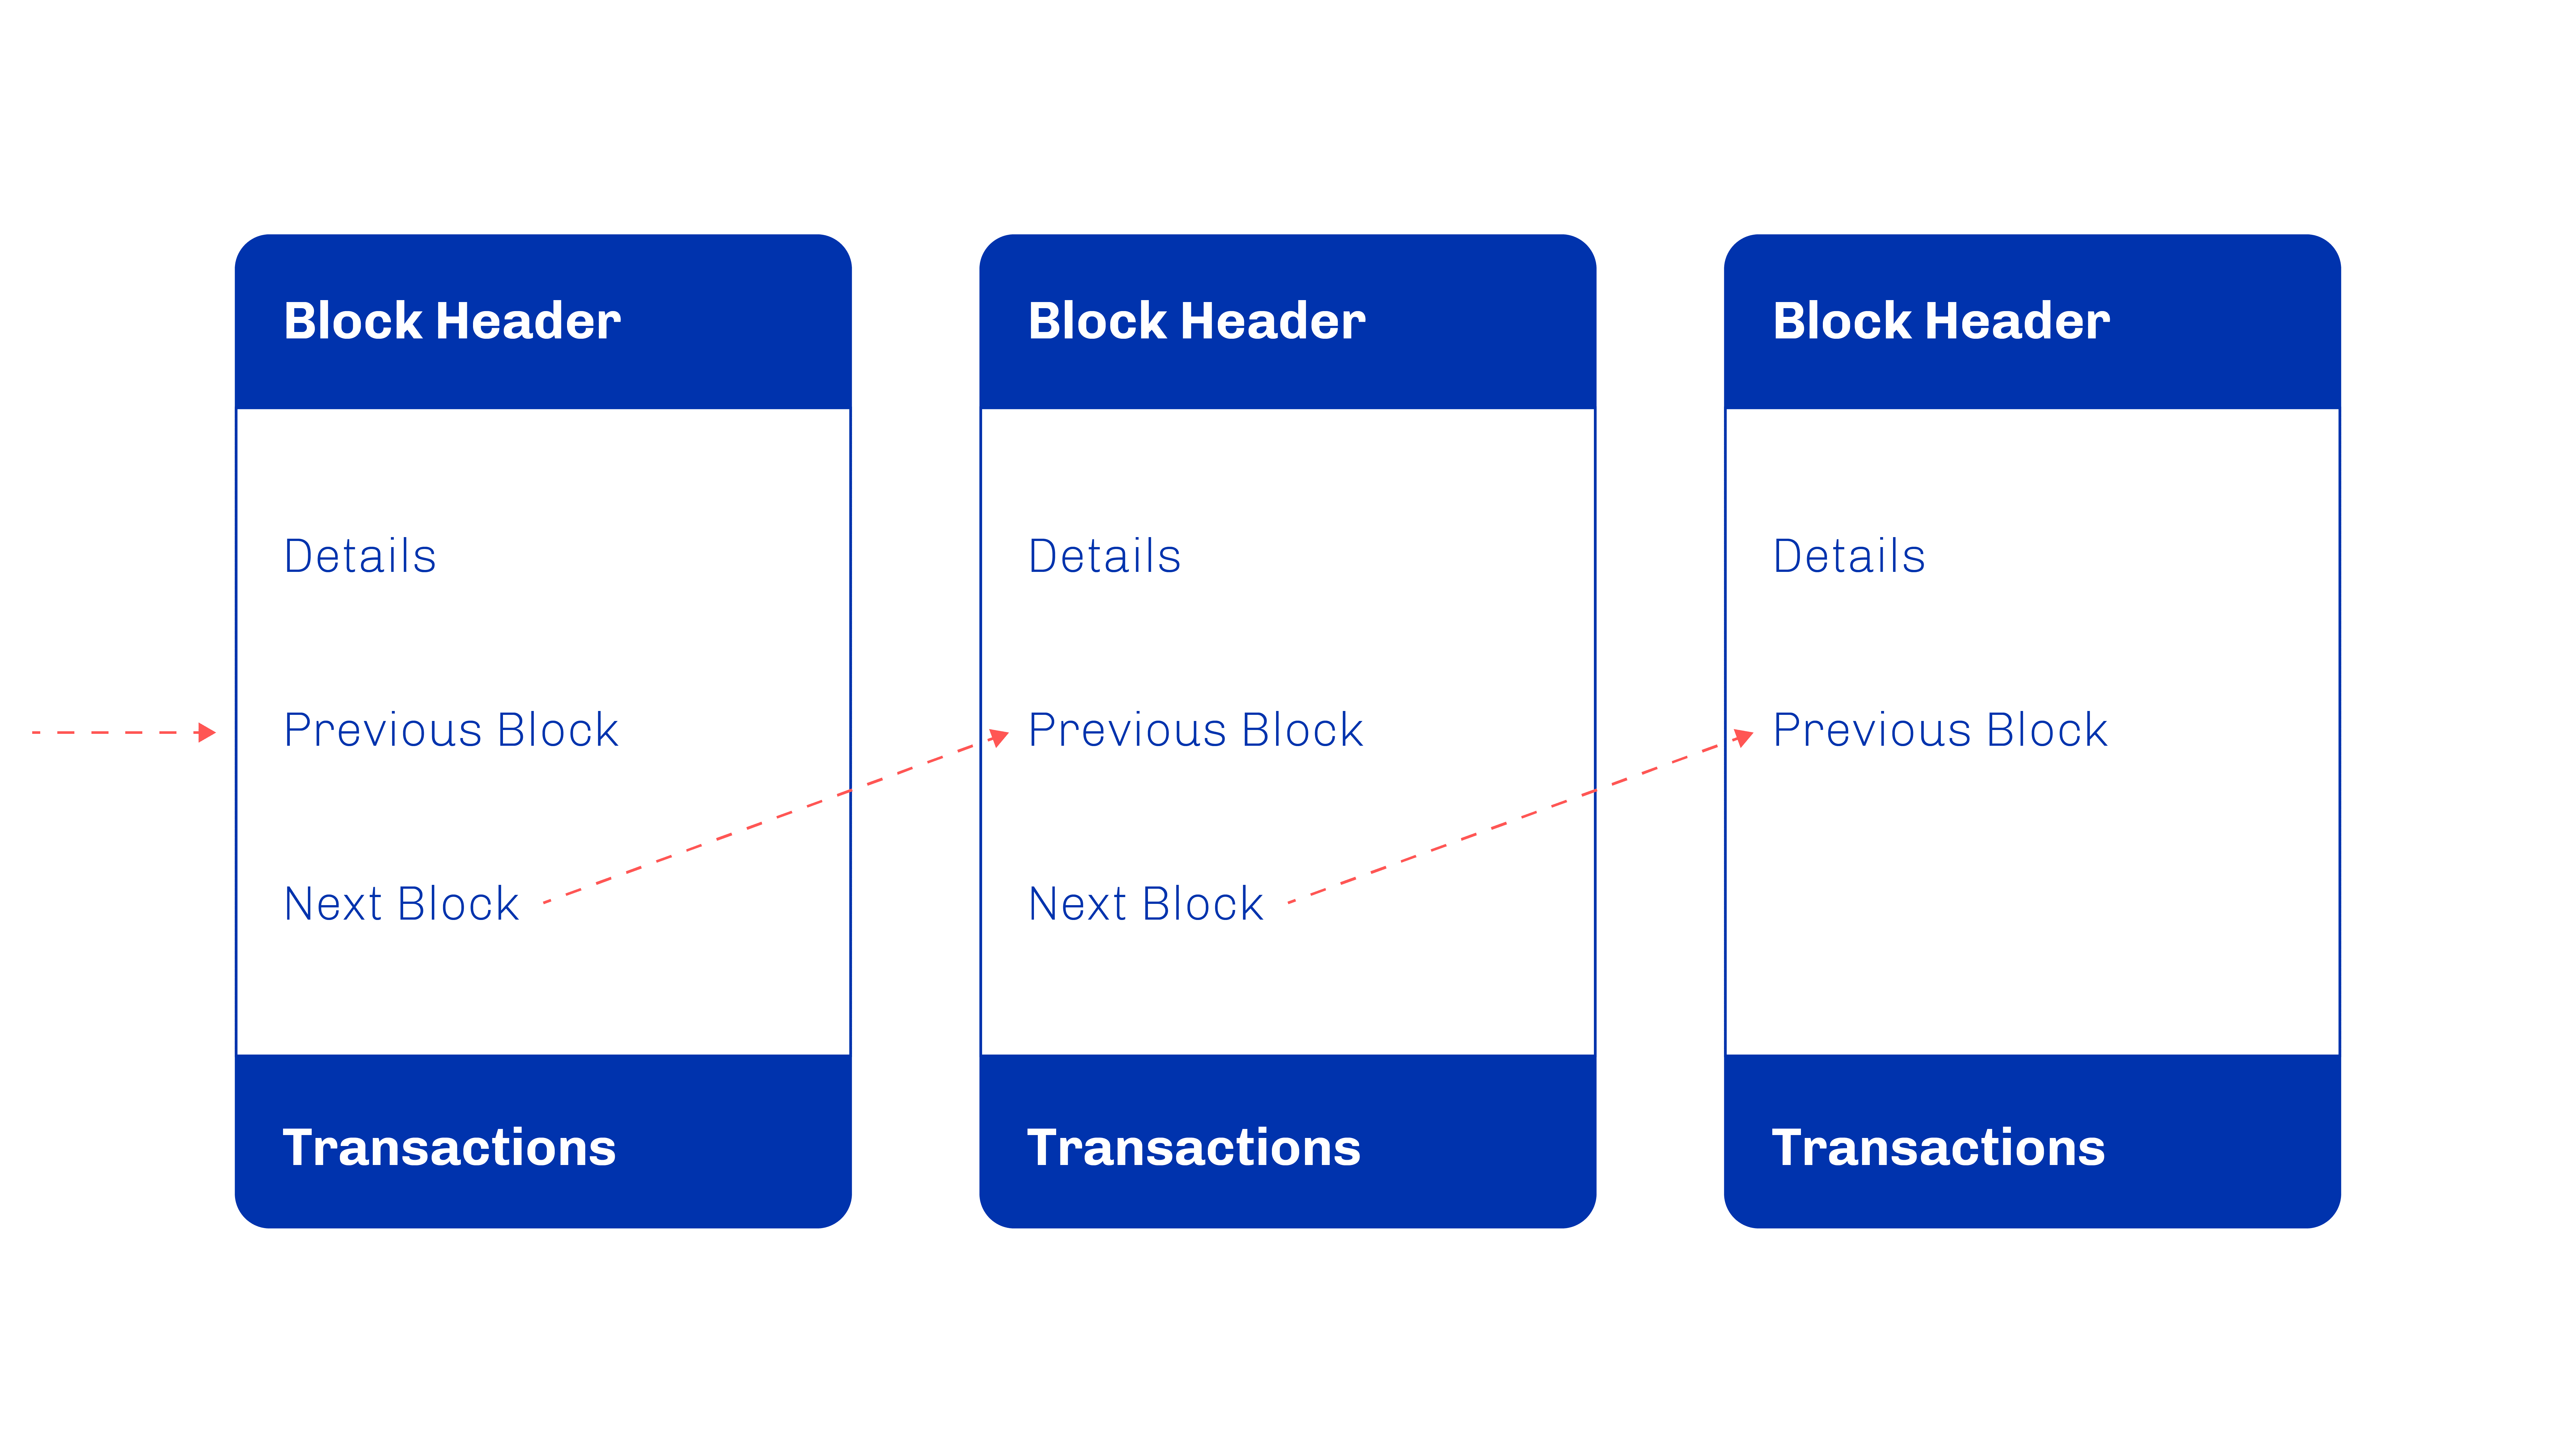
\includegraphics[width=0.9\textwidth]{Bloques.png}
    \caption[Representación simplificada de los datos en un bloque de la cadena.]{Representación simplificada de los datos en un bloque de la cadena. Extraída de~\cite{plutus-smart-contracts}.}\label{fig:Bloques}
\end{figure}


\end{frame}

\begin{frame}{Criptomonedas}
Las \underline{criptomonedas} son \textbf{activos digitales que se almacenan en el ledger} y están diseñadas para servir como medio de intercambio de bienes o servicios. 

\pause
\vfill

Las blockchain son utilizadas como \textbf{tecnología subyacente} para la creación de criptomonedas en un entorno descentralizado. 

\pause
\vfill

La creación, seguridad y verificación de las criptomonedas y transacciones son propiedades que debe garantizar la blockchain correspondiente.

\pause
\vfill

El precio de la criptomoneda no está controlado por un gobierno o una institución financiera centralizada.

\end{frame}

\begin{frame}{\textit{Smart contracts}}
Un contrato inteligente (\textit{smart contract}) es un \textbf{acuerdo digital automatizado}.

\pause
\vfill

Están escritos en código y \textbf{rastrean, verifican y ejecutan las transacciones de un contrato} entre varias partes.

\pause
\vfill

Las transacciones del contrato se ejecutan automáticamente cuando se cumplen las condiciones predeterminadas. Esencialmente, \textbf{un contrato inteligente es un programa cuyas entradas y salidas son acciones en una cadena de bloques}.

\pause
\vfill

Los smart contracts no requieren las acciones o la presencia de terceros. El código del contrato inteligente se almacena y distribuye en la \textit{blockchain}, lo que lo hace \textbf{transparente e irreversible}.

\end{frame}

\subsection{Cardano}

{\nologo
\begin{frame}
Cardano es una plataforma blockchain descentralizada de tercera generación, cuya criptomoneda es llamada \textit{ada}. 

\vfill
\pause

\begin{itemize}
    \item \textbf{La primera generación} de blockchains (por ejemplo Bitcoin) ofrece ledgers descentralizados para la transferencia segura de criptomonedas. 
    \smallskip

    \pause Sin embargo, tales \textit{blockchains} no proporcionaron un entorno funcional para la liquidación de acuerdos complejos.
    \pause
    \vfill

    \item \textbf{La segunda generación} (por ejemplo Ethereum) proporcionó soluciones mejoradas para redactar y ejecutar contratos inteligentes, desarrollar aplicaciones y crear diferentes tipos de tokens.
    \smallskip

    \pause Sin embargo, la segunda generación de cadenas de bloques a menudo enfrenta problemas en términos de escalabilidad.
\end{itemize}
\end{frame}
}

\begin{frame}{Cardano como \textit{blockchain} de 3ra generación}

Combina las propiedades de las generaciones anteriores y ofrece las siguientes propiedades:
\vfill
\pause

\begin{itemize}
    \item \textbf{Escalabilidad}: Rendimiento de transacciones, escala de datos y ancho de banda de la red.
        \pause
    \item \textbf{Funcionalidad}: Además del procesamiento de transacciones, la cadena de bloques proporciona todos los medios para la liquidación de acuerdos comerciales. 
        \pause
    \item \textbf{Desarrollo e Integración}: Es sencillo integrar pagos con otras cadenas.
\end{itemize} 

\end{frame}


\begin{frame}{Ada como criptomoneda de Cardano}
Ada es la moneda nativa o principal en Cardano. Esto significa que ada es la principal unidad de pago.

\pause
\vfill

Sin embargo, también admite la creación de \textbf{tokens nativos}: activos digitales que se crean para fines
específicos. 

\vfill
\pause

Esto permite a los usuarios, desarrolladores y empresas usar a Cardano para crear tokens que representen valor.

\pause
\vfill

Un token puede ser \textbf{fungible} (intercambiable) o \textbf{no fungible} (único) y actuar como unidad de pago, recompensa, activo comercial o contenedor de información.

\end{frame}

\begin{frame}{El lenguaje Marlowe}
    Marlowe es un lenguaje de dominio específico creado por IOHK. El mismo posee \textbf{pocas sentencias que describen el comportamiento de un conjunto fijo y finito de roles en un contrato}.

\vfill
Los contratos se pueden construir reuniendo una pequeña cantidad de estas sentencias que se pueden usar para \textbf{describir y modelar contratos financieros}. 
\vfill

\pause
Algunos ejemplos incluyen:
\begin{itemize}
    \item Un contrato que puede realizar un pago a un rol o a una clave pública
    \item Un contrato que puede esperar una acción por parte de uno de los roles:
        \begin{itemize}
            \item Un depósito de moneda.
            \item Una elección entre un conjunto de opciones.
        \end{itemize}
\end{itemize}

\end{frame}



\subsection{ACTUS}

\begin{frame}{Contratos Financieros}
Los contratos financieros son \textbf{acuerdos legales entre dos (o más) partes} sobre el \textbf{futuro intercambio de dinero}. 

\vfill

Dichos acuerdos legales se definen sin ambigüedades por medio de un conjunto de términos y lógica contractual.

\pause
\vfill

Como resultado, los mismos pueden describirse matemáticamente y representarse mediante algoritmos.

\end{frame}

%\begin{frame}
%Los beneficios de representar contratos financieros de esta forma son múltiples:

%\begin{itemize}
    %\pause

    %\item Tradicionalmente, el procesamiento de transacciones ha sido un campo en el que se pueden lograr mejoras de eficiencia mediante la automatización de contratos.

    %\pause

    %\item El análisis financiero se basa en la disponibilidad de representaciones computables de estos acuerdos, donde a menudo se utilizan aproximaciones analíticas. \pause Recientemente, el auge de las blockchain, de contabilidad distribuida y los diversos casos de uso de los contratos inteligentes han abierto nuevas posibilidades para los contratos financieros digitales.
%\end{itemize}

%\end{frame}

\begin{frame}
    En general, \textbf{el intercambio de flujos de efectivo} entre partes \textbf{sigue ciertos patrones}. \pause
    \vfill

    Un patrón típico es un contrato de préstamo: \pause

    \vfill

    \begin{quote}
        ``Se entrega un monto de dinero inicial, a cambio de pagos de intereses cíclicos y la devolución del dinero inicial en el vencimiento del contrato.''
    \end{quote}
    \pause
    \vfill

    Si bien los pagos son fijos, \textbf{existen muchas variantes} que determinan cómo se programan y/o pagan los pagos de intereses cíclicos:
    \begin{itemize}
        \pause
        \item Los pagos de intereses pueden ser mensuales, anuales, mediante períodos arbitrarios. 
        \pause
        \item Las tasas pueden ser de fijas o variables.
        \pause
        \item Pueden usarse diferentes métodos de cálculo de fracciones anuales o que no haya ningún interés.
    \end{itemize}

\end{frame}

\begin{frame}[fragile]
\begin{figure}[H]
    \centering
    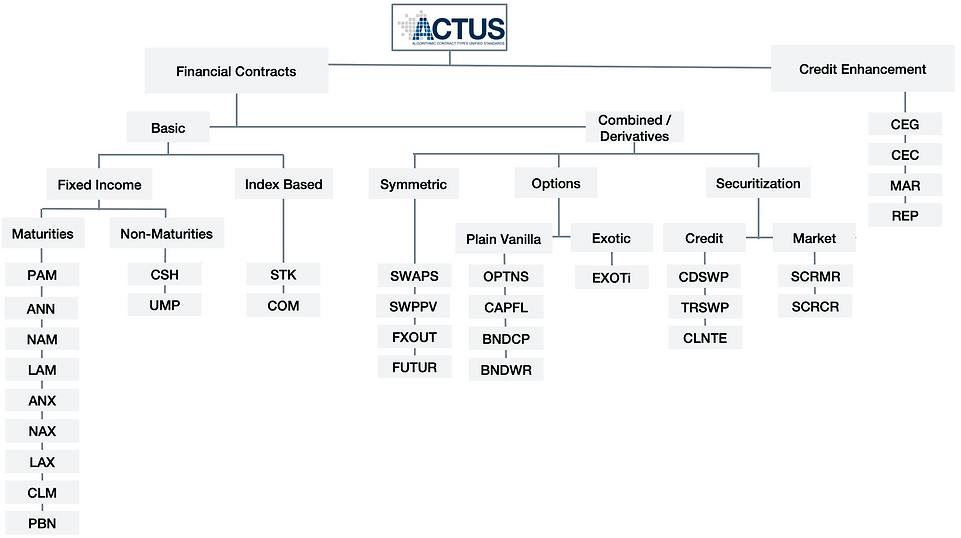
\includegraphics[width=\textwidth]{ACTUS_Taxonomy.png}
    \caption{Taxonomía ACTUS}
\end{figure}

\end{frame}



\subsection{Verificación formal de software}

\begin{frame}{Concepto general, herramientas y metodologías}
Los asistentes de pruebas formales son herramientas de software diseñadas para ayudar a sus usuarios a realizar pruebas, especialmente en cálculo lógico.

\vfill
\pause

A diferencia de los tests convencionales, durante una verificación \textbf{no se ejecuta el programa a analizar}, es por eso que este tipo de análisis es denominado \textbf{estático}.

\vfill

Cuando un teorema es escrito y probado, el mismo debe será verdadero para cualquier combinación de las variables de entrada.

\vfill
\pause

La principal fortaleza de los asistentes es que ayudan a desarrollar \textbf{pruebas altamente confiables e inequívocas} de enunciados matemáticos y algoritmos, usando lógica precisa.
\end{frame}

\begin{frame}{Algunos asistentes de pruebas}

A continuación presentamos una lista de los principales, clasificados por sus fundamentos lógicos:
\vfill
\pause

\begin{itemize}
    \item \textbf{Teoría de conjuntos}: Isabelle/ZF, Metamath, Mizar
    \item \textbf{Teoría simple de tipos}: HOL4, HOL Light, \only<2>{Isabelle/HOL}\only<3>{\hl{Isabelle/HOL}}
    \item \textbf{Teoría dependiente de tipos}: Agda, Coq, Lean, Matita, PVS
    \item \textbf{Lógica de primer orden, de tipo Lisp}: ACL2
\end{itemize}
\end{frame}

\section{Escribiendo contratos ACTUS en Cardano}

\subsection{Notación del estándar ACTUS}

{\nologo
\begin{frame}{Notación}
\begin{itemize}
    \item \textbf{\underline{Atributos de contrato}}: Representan los términos contractuales que definen el flujo de dinero en un contrato financiero.
    \pause
\item \textbf{\underline{Starting date}}: $t_0$ representa la fecha de comienzo del contrato, y marca el instante en el cual las condiciones y estado del contrato están siendo representados. 
    \pause
    \item \textbf{\underline{Variables de estado}}: Las variables de estado describen el estado de un contrato, para un tiempo determinado de su ciclo de vida. 

        Algunos ejemplos de las mismas son: 
        \pause
            \begin{itemize}
                \item \textbf{Accrued Interest (IPAC)}: Interés acumulado en `\textit{Status date}' (SD).
                \item \textbf{Performance (PRF)}: Estado actual del contrato (\textit{performant}, \textit{delayed}, \textit{terminated}, etc.)
            \end{itemize}
        \pause
        En general, el ‘estado’ representa ciertos atributos que pueden cambiar durante su ciclo de ejecución, de acuerdo a eventos programados o no programados. 
\end{itemize}
\end{frame}
}

\begin{frame}
    \begin{itemize}
        \item \textbf{\underline{Eventos}}: Un evento de contrato $e_t^k$ se refiere a cualquier evento \textit{programado} o \textit{no programado} en un momento determinado $t$ y de un tipo determinado $k$. 
        \vfill

        Los eventos del contrato \textbf{marcan puntos específicos} en el tiempo en el que se \textbf{intercambian flujos de efectivo} o se \textbf{actualiza el estado del contrato}. 

        \vfill
        \pause

        Algunos tipos de eventos:

        \begin{itemize}
            \item \textbf{AD}: Monitoreo del contrato.
            \item \textbf{IP}: Pago de interés programado.
            \item \textbf{IPCI}: Capitalización de interés programada.
            \item \textbf{PRD}: Compra de un contrato.
            \item \textbf{TD}: Terminación de un contrato.

        \end{itemize}
    \end{itemize}
\end{frame}

\begin{frame}
    \begin{itemize}
        \item \textbf{Funciones de transición de estado} (\textit{State Transition Functions} o STF): definen la transición de las variables de estado desde el \textit{pre-evento} hacia el \textit{post-evento}, cuando un cierto evento $e^k_t$ ocurre. 

            Esto provoca que el \textit{pre-evento} y \textit{post-evento} reciban la notación de $t^-$ y $t^+$ respectivamente.

  \end{itemize}
  \pause
  \vfill
  Estas funciones son específicas para un tipo de evento y contrato. Su notación es de la forma $\textbf{STF\_[event type]\_[contract type]()}$.
  \vfill
  \pause

  Por ejemplo: La STF para un evento de tipo IP en el contrato PAM se escribe como $\text{STF\_IP\_PAM ()}$ y modifica (entre otras) a la variable $\textbf{Ipac}$ desde el pre-evento $\textbf{Ipac}_{t^-}$ al post-evento $\textbf{Ipac}_{t^+}$.

\end{frame}

{\nologo
\begin{frame}[fragile]
    \begin{itemize}
        \item \textbf{Funciones de pago} (\textit{Payoff Functions} o POF): definen como el flujo de dinero $c \in\mathbb{R}$ ocurre para un determinado evento $e^k_t$. 

            El mismo es obtenido del estado actual y los términos del contrato. Si fuera necesario, el flujo de dinero puede ser indexado con el tiempo del evento: $c_t$.
    \end{itemize}
    \pause
    \vfill

    Las funciones de pago son específicas para un tipo de evento y contrato, y su notación es la siguiente: $\textbf{POF\_[event type]\_[contract type] ()}$.
    \vfill
    \pause

    \begin{figure}[H]
        \centering
        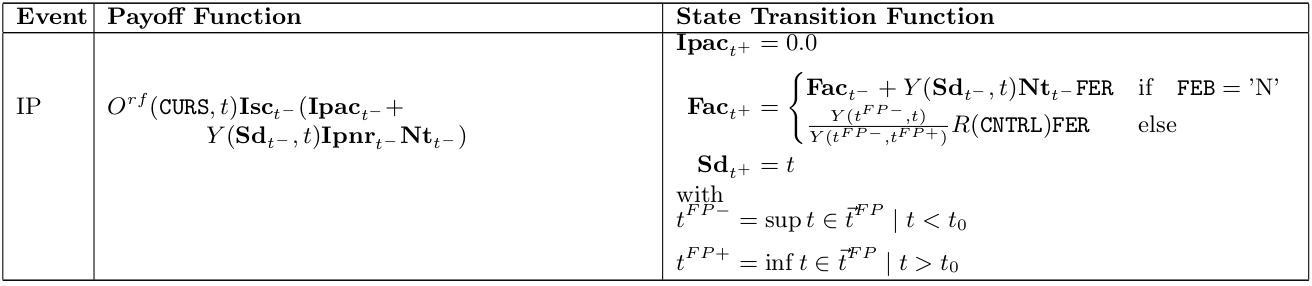
\includegraphics[width=\textwidth]{POF_STF_IP_PAM.png}
    \end{figure}

\end{frame}
}

\subsection{Contratos en Cardano}

{\nologo
\begin{frame}{Introducción}
En esta sección describiré la estructura de 3 contratos ACTUS que escribí para la blockchain Cardano, bajo la supervisión de IOHK.\@

\vfill
\pause

Agregar contratos ACTUS en la blockchain Cardano implica agregar, para cada contrato:

\begin{itemize}
        \pause
    \item Scheduling.
        \pause
    \item Inicialización de variables de estado.
        \pause
    \item Funciones de transición de estado y de pago, para cada evento relevante.
        \pause
    \item Validación mediante los tests propuestos por el estándar ACTUS.
\end{itemize}

\pause
\vfill

Dicho código fue incorporado en la rama principal del repositorio de \href{https://github.com/input-output-hk/marlowe-cardano}{marlowe-cardano}. Por lo que usuarios podrán utilizar dichos contratos en el futuro.
\end{frame}
}

\begin{frame}[fragile]{Estructura del proyecto ACTUS en Cardano}
A grandes rasgos, la estructura del generador de contratos ACTUS tiene los siguientes módulos:
    \vfill
    
\begin{itemize}
    \item  \textbf{\underline{Domain}}: El mismo está conformado por los archivos que modelan el dominio de los contratos ACTUS.

        \medskip

        En este módulo podemos encontrar los tipos de \textbf{eventos}, \textbf{términos} y el \textbf{Estado} del contrato, entre otros.
        \pause
        \vfill

    \item \textbf{\underline{Generator}}: Se implementan los diferentes generadores y compatibilidad hacia el lenguaje Marlowe. 

        \medskip

        Dichos generadores se utilizan para obtener código en Marlowe, Javascript, Haskell o Blockly, y pueden generar contratos estáticos (sin riesgos o eventos externos).
\end{itemize}
\end{frame}


\begin{frame}
    \begin{itemize}
        \item \textbf{\underline{Model}}: Se encuentra la lógica expuesta por el estándar ACTUS. 

            \medskip

            Este módulo es responsable del \textbf{scheduling}, la \textbf{inicialización de variables de estado} y \textbf{funciones de transición de estado y de pago}.

            \vfill
            \pause

        \item \textbf{\underline{Utility}}: Se encuentran algunos módulos con funciones que se utilizan para aislar la lógica del \textbf{cálculo y convenciones de fechas}, que suele tornarse complejo y repetitivo durante los contratos.
    \end{itemize}
\end{frame}

{\nologo
\begin{frame}[fragile]
\only<1>{
    \begin{figure}[H]
        \centering
        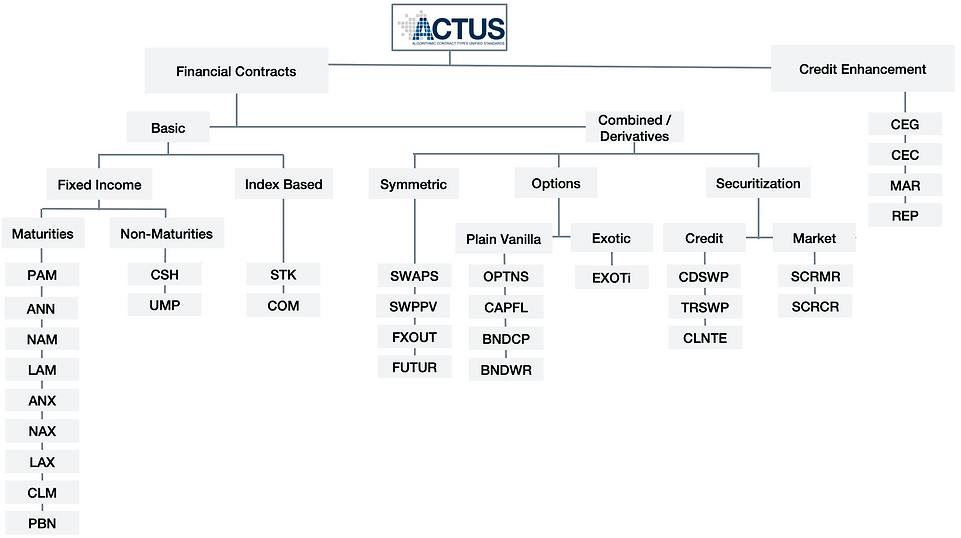
\includegraphics[width=\textwidth]{ACTUS_Taxonomy.png}
        \caption{Taxonomía ACTUS}
    \end{figure}
\vspace{0.70mm} 
}

\only<2>{
    \begin{figure}[H]
        \centering
        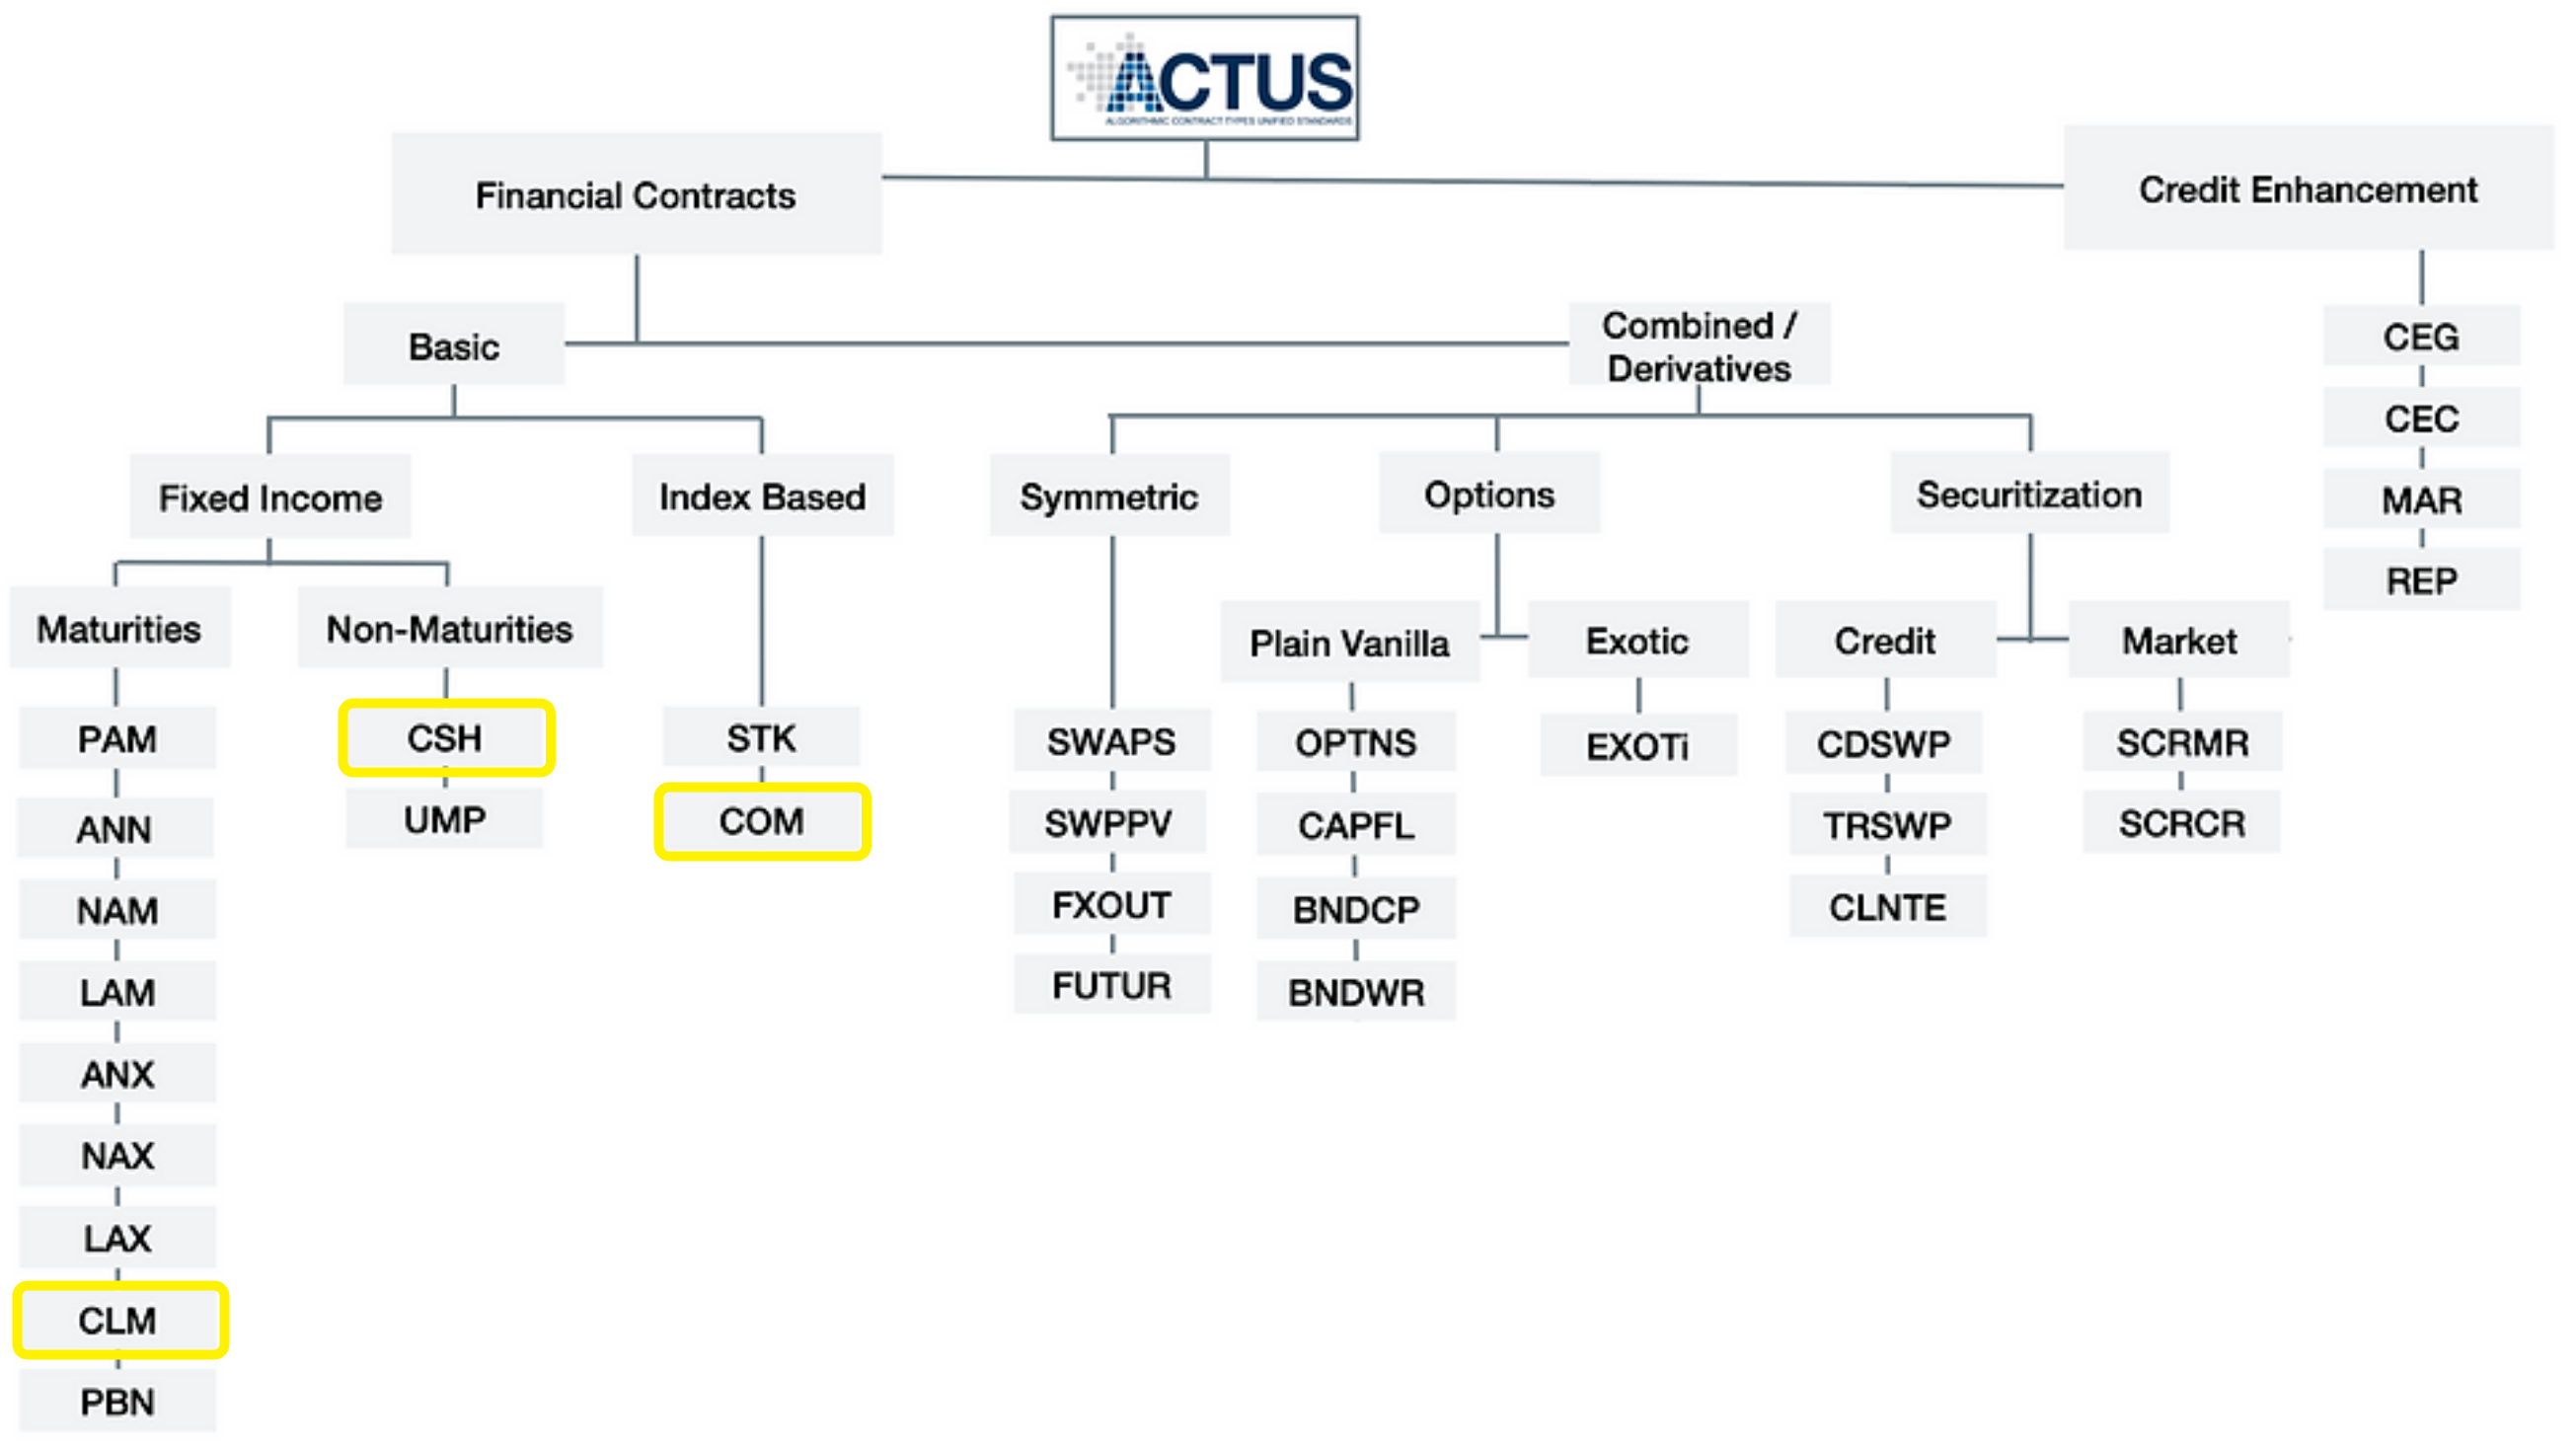
\includegraphics[width=\textwidth]{ACTUS_Taxonomy_hl.png}
        \caption{Contratos que implementé como parte del desarrollo de mi tesis}
    \end{figure}
}
\end{frame}
}

{\nologo
\begin{frame}[fragile]{Fragmentos de los contratos que implementé}

Especificación ACTUS:

\begin{figure}[H]
    \centering
    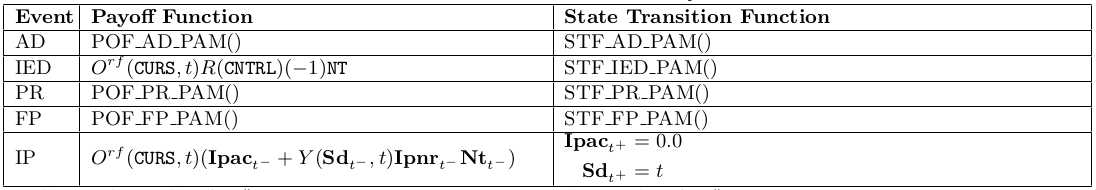
\includegraphics[width=\textwidth]{POF_CLM.png}
\end{figure}

Implementación para Cardano:
\begin{code}{Haskell-cardano}
-- Call Money (CLM) POF's

_POF_IP_CLM :: ActusNum a => a -> a -> a -> a -> a -> a
_POF_IP_CLM o_rf_curs ipac ipnr nt y_sd_t = o_rf_curs * (ipac + y_sd_t * ipnr * nt)

_POF_IED_CLM :: RoleSignOps a => a -> CR -> a -> a
_POF_IED_CLM o_rf_curs cntrl nt = _zero - o_rf_curs * _r cntrl * nt


\end{code}
\end{frame}
}

{\nologo
\begin{frame}[fragile]
\begin{figure}[H]
    \centering
    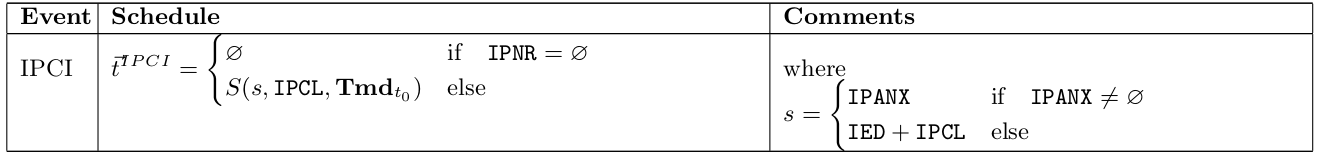
\includegraphics[width=\textwidth]{Schedule_CLM.png}
\end{figure}

\vspace{-5.00mm} 

\begin{code}{Haskell-cardano}
_SCHED_IP_CLM
  ContractTermsPoly
    { cycleAnchorDateOfInterestPayment = Just ipanx,
      cycleOfInterestPayment = Just ipcl,
      maturityDate = Just md,
      scheduleConfig
    } = generateRecurrentSchedule ipanx ipcl {includeEndDay = True} md scheduleConfig

_SCHED_IP_CLM
  ContractTermsPoly
    { cycleAnchorDateOfInterestPayment = Nothing,
      cycleOfInterestPayment = Just ipcl,
      maturityDate = Just md,
      initialExchangeDate = Just ied,
      scheduleConfig
    } = generateRecurrentSchedule (ied <+> ipcl) ipcl {includeEndDay = True} md scheduleConfig
\end{code}

\end{frame}
}

{\nologo
\begin{frame}[fragile]{STF para el contrato CSH y el evento AD (Monitoring)}

\begin{figure}[H]
    \centering
    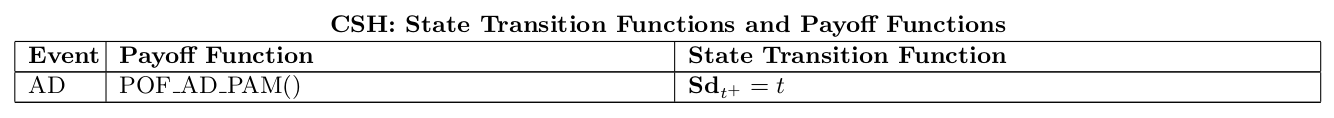
\includegraphics[width=\textwidth]{CSH_STF.png}
\end{figure}

\vfill

\begin{code}{Haskell-cardano}
-- Cash (CSH) Monitoring STF 
_STF_AD_CSH :: ContractStatePoly a b -> b -> ContractStatePoly a b
_STF_AD_CSH st@ContractStatePoly {} t =
  st
    { sd = t
    }
\end{code}

\end{frame}
}


\section{Verificando propiedades en contratos en Marlowe}

\subsection{El modelo de Marlowe}

\begin{frame}{El modelo de Marlowe}
Marlowe está diseñado para soportar la ejecución de contratos financieros en la blockchain, específicamente en Cardano.

\vfill
\pause

Antes de describir estos constructores, debemos analizar el enfoque general para \textbf{modelar contratos en Marlowe}, el contexto y las partes involucradas cuando se ejecutan los mismos.

\end{frame}

{\nologo
\begin{frame}[fragile]
\begin{itemize}
    \item Contratos
        \pause

\begin{code}{Haskell-Cardano}
data Contract = Close
              | Pay party payee token value contract
              | If observation contract1 contract2
              | When [Case] timeout contract
              | Let valueId value contract
              | Assert observation contract
\end{code}
        \pause
    \item Participantes y roles
        \pause
    \item Valores y \textit{tokens}
        \pause
    \item Cuentas
        \pause
    \item Pasos y Estados
        \pause
    \item Simulación omnisciente (\textit{Marlowe Playground})

\end{itemize}
\end{frame}
}

{\nologo
\begin{frame}[fragile]{Breve ejemplo de un contrato de Intercambio}
\begin{code}{Haskell-Cardano}
When [Case (Deposit "alice" "alice" ada price)   
        (When [ Case aliceChoice
                  (When [ Case bobChoice
                            (If (aliceChosen `ValueEQ` bobChosen)
                                 agreement
                                 arbitrate) 
                        ]
                        60 -- Slot limite para la eleccion de Bob
                        arbitrate)
              ]
              40  -- Slot limite para la eleccion de Alice
              Close)
     ]
     10   -- Slot limite para el Deposito
     Close    

-- agreement y arbitrate son contratos auxiliares que realizan los pagos o devoluciones correspondientes
\end{code}

\end{frame}
}

\begin{frame}{Ejecución de un contrato Marlowe}

Ejecutar un contrato de Marlowe en la cadena de bloques de Cardano significa restringir las transacciones generadas por el usuario a la lógica del contrato.
\vfill
\pause

Una \textbf{transacción} contiene una \textbf{lista ordenada de \textit{entradas} o \textit{acciones}}. El intérprete de Marlowe se ejecuta durante la validación de transacciones. 

\end{frame}

\begin{frame}{Procesando una transacción}
\begin{enumerate}
    \item Se evalúa (o reduce) el contrato \textit{paso} a \textit{paso} hasta que \textbf{no se puede cambiar más sin procesar alguna entrada}, una condición que se llama \textit{quiescent} (o inactiva).

    \medskip
    Esto implica reducir los \texttt{When} cuyos timeouts hayan sido superados, y todos los constructores \texttt{If}, \texttt{Let}, \texttt{Pay} y \texttt{Close}.

    \vfill
    \pause

    \item Se procesa (o aplica) la primera entrada y luego el contrato se vuelve a procesar hasta la inactividad. 
\end{enumerate}
\vfill
\pause
Este proceso se repite \textbf{hasta que se procesan todas las entradas}. En cada paso, \textbf{el contacto actual y el estado cambiarán} y es posible que se realicen pagos.
\end{frame}

\begin{frame}

\begin{figure}[H]
    \centering
    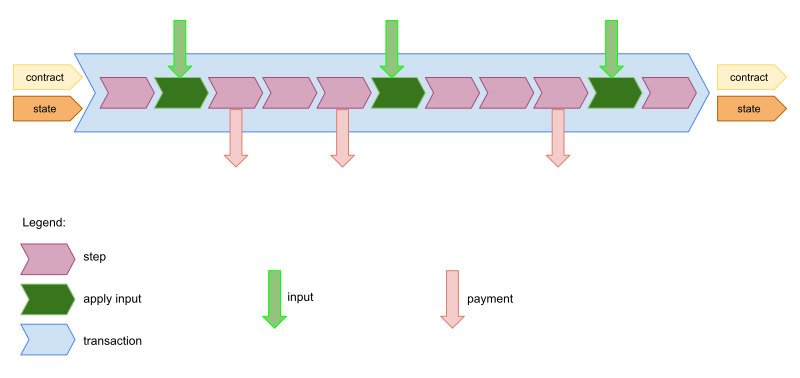
\includegraphics[width=\textwidth]{Transaccion.png}
    \caption[Diagrama de ejemplo de una transacción.]{Diagrama de ejemplo de una transacción. Extraído de \href{https://play.marlowe-finance.io/doc/marlowe/tutorials/marlowe-model.html}{la documentación oficial del Modelo de Marlowe}.}\label{fig:Transaccion}
\end{figure}

\end{frame}

{\nologo
\begin{frame}[fragile]{Funciones utilizadas en el modelo}

\only<1>{
    \begin{figure}[H]
        \centering
        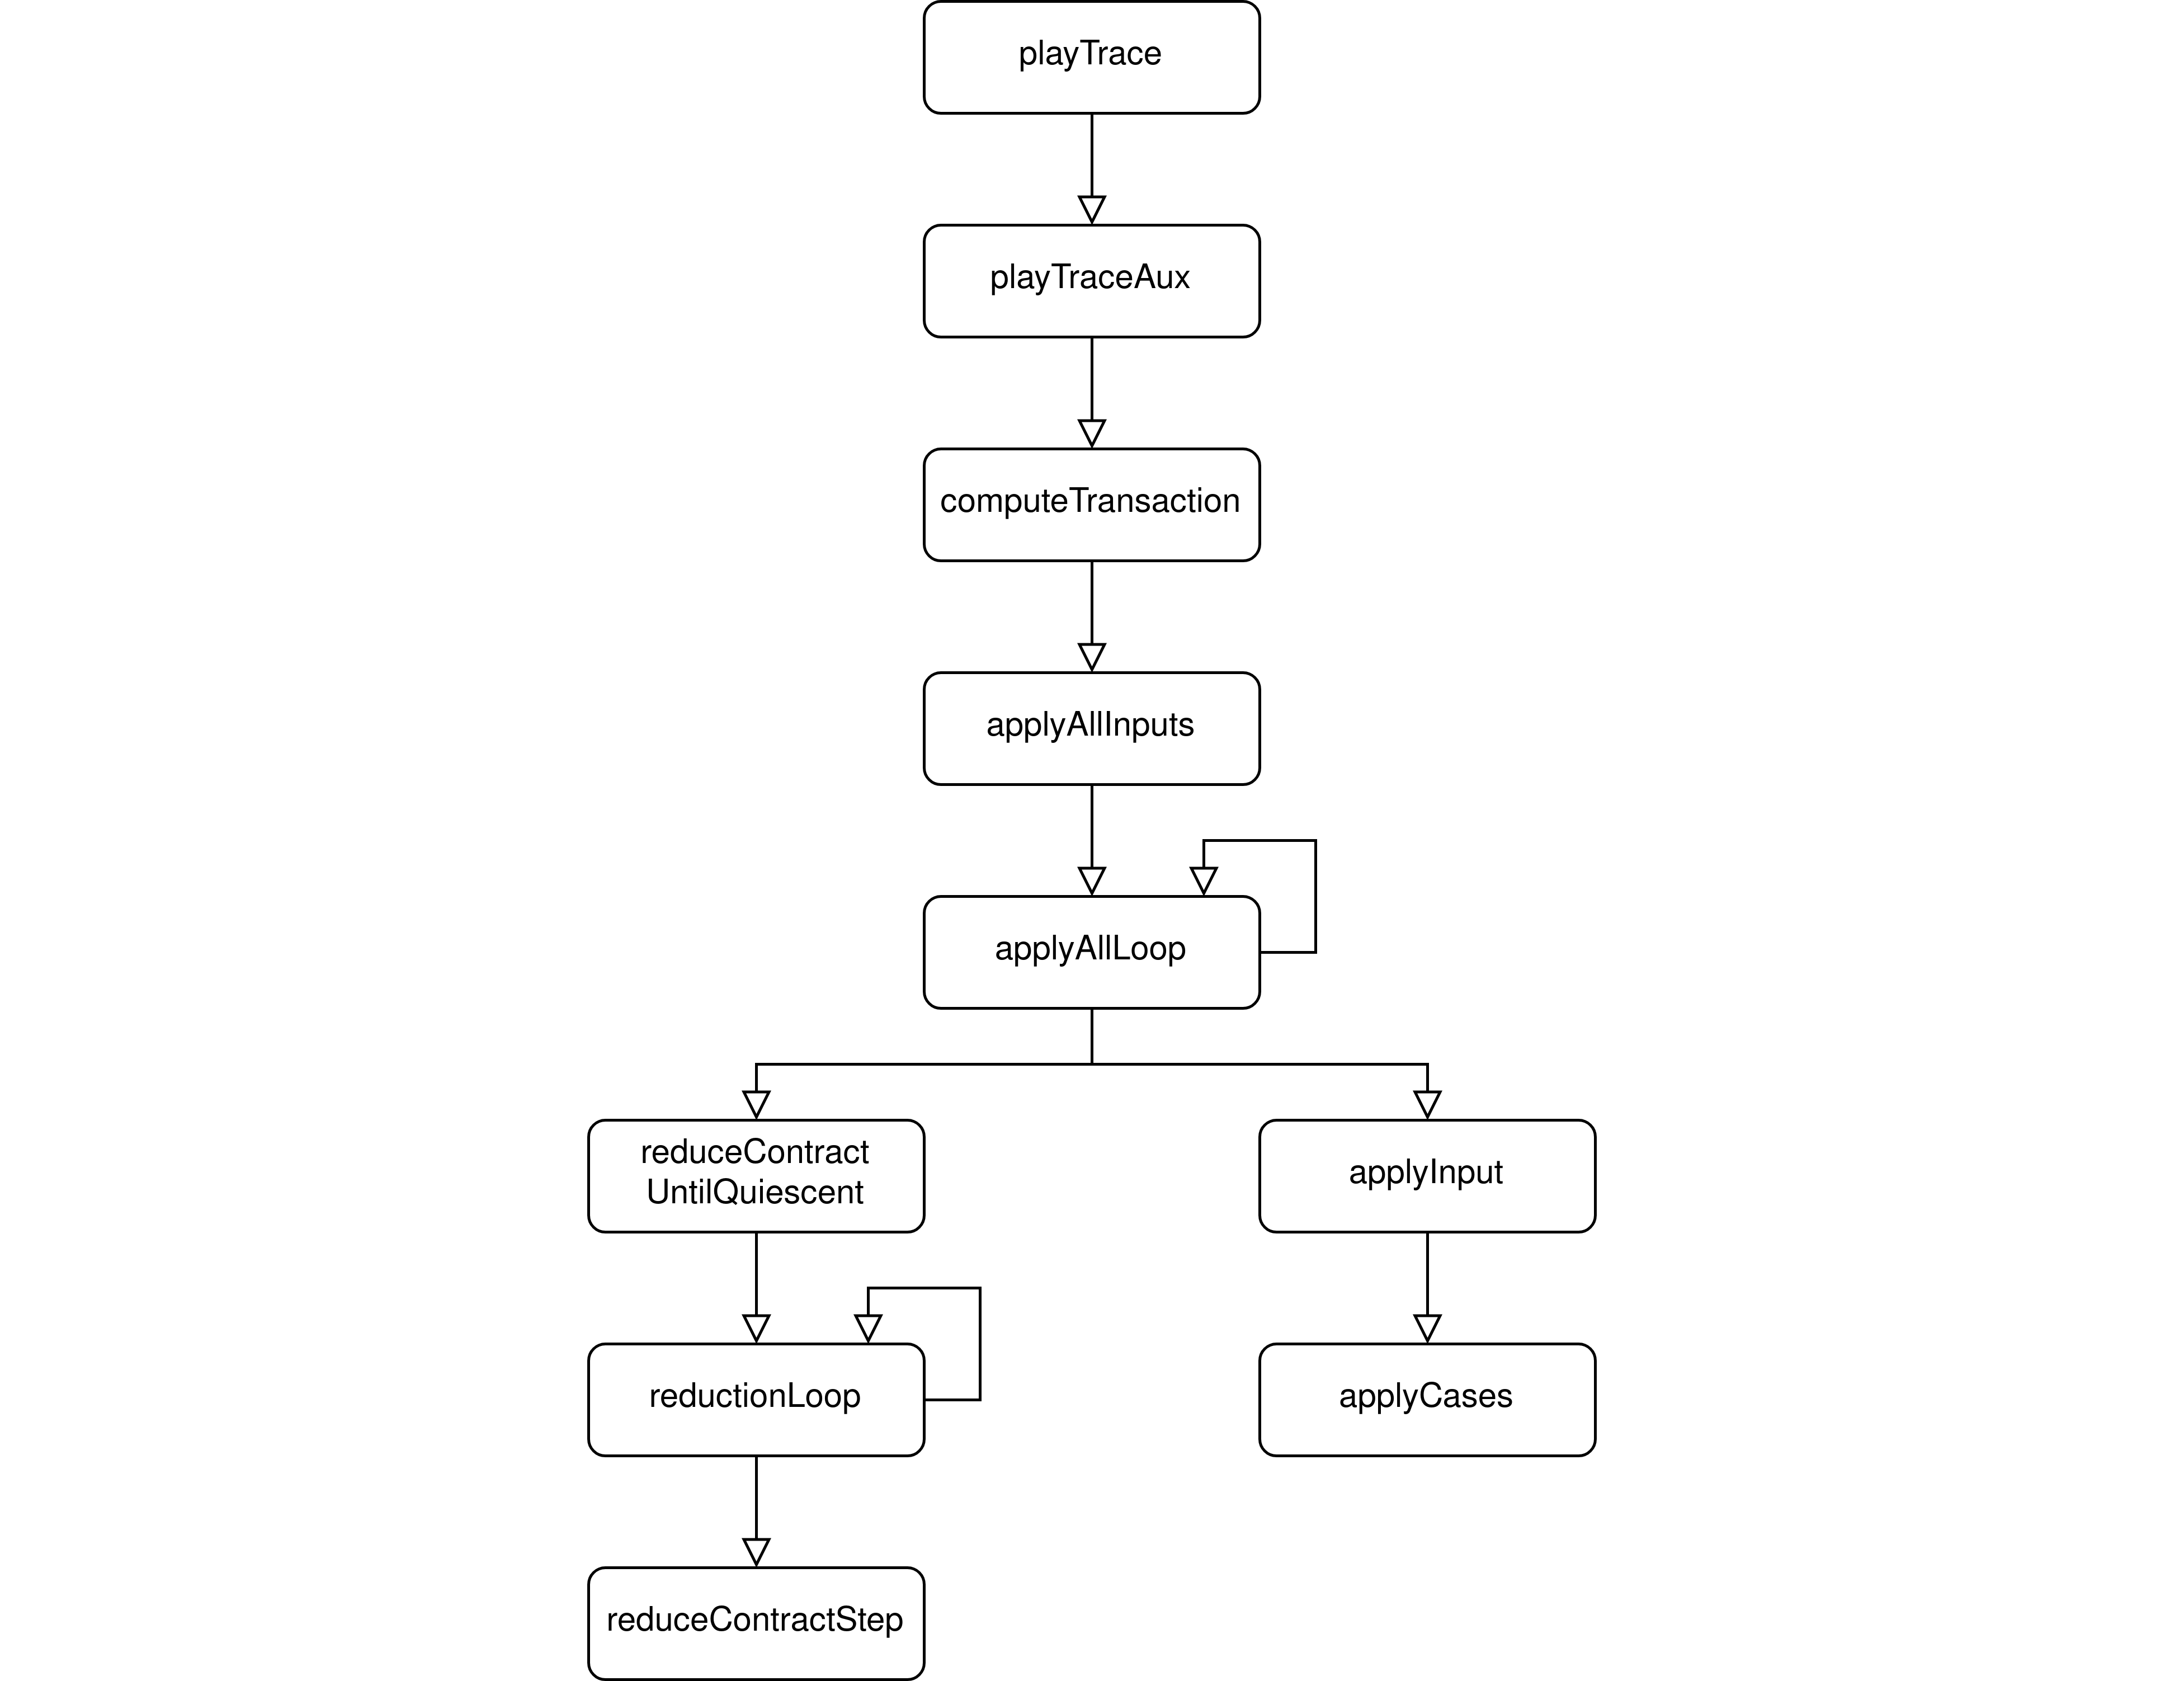
\includegraphics[height=0.8\textheight]{Dependencias_Isabelle_Marlowe.png}
    \end{figure}
}
\only<2>{
    \begin{figure}[H]
        \centering
        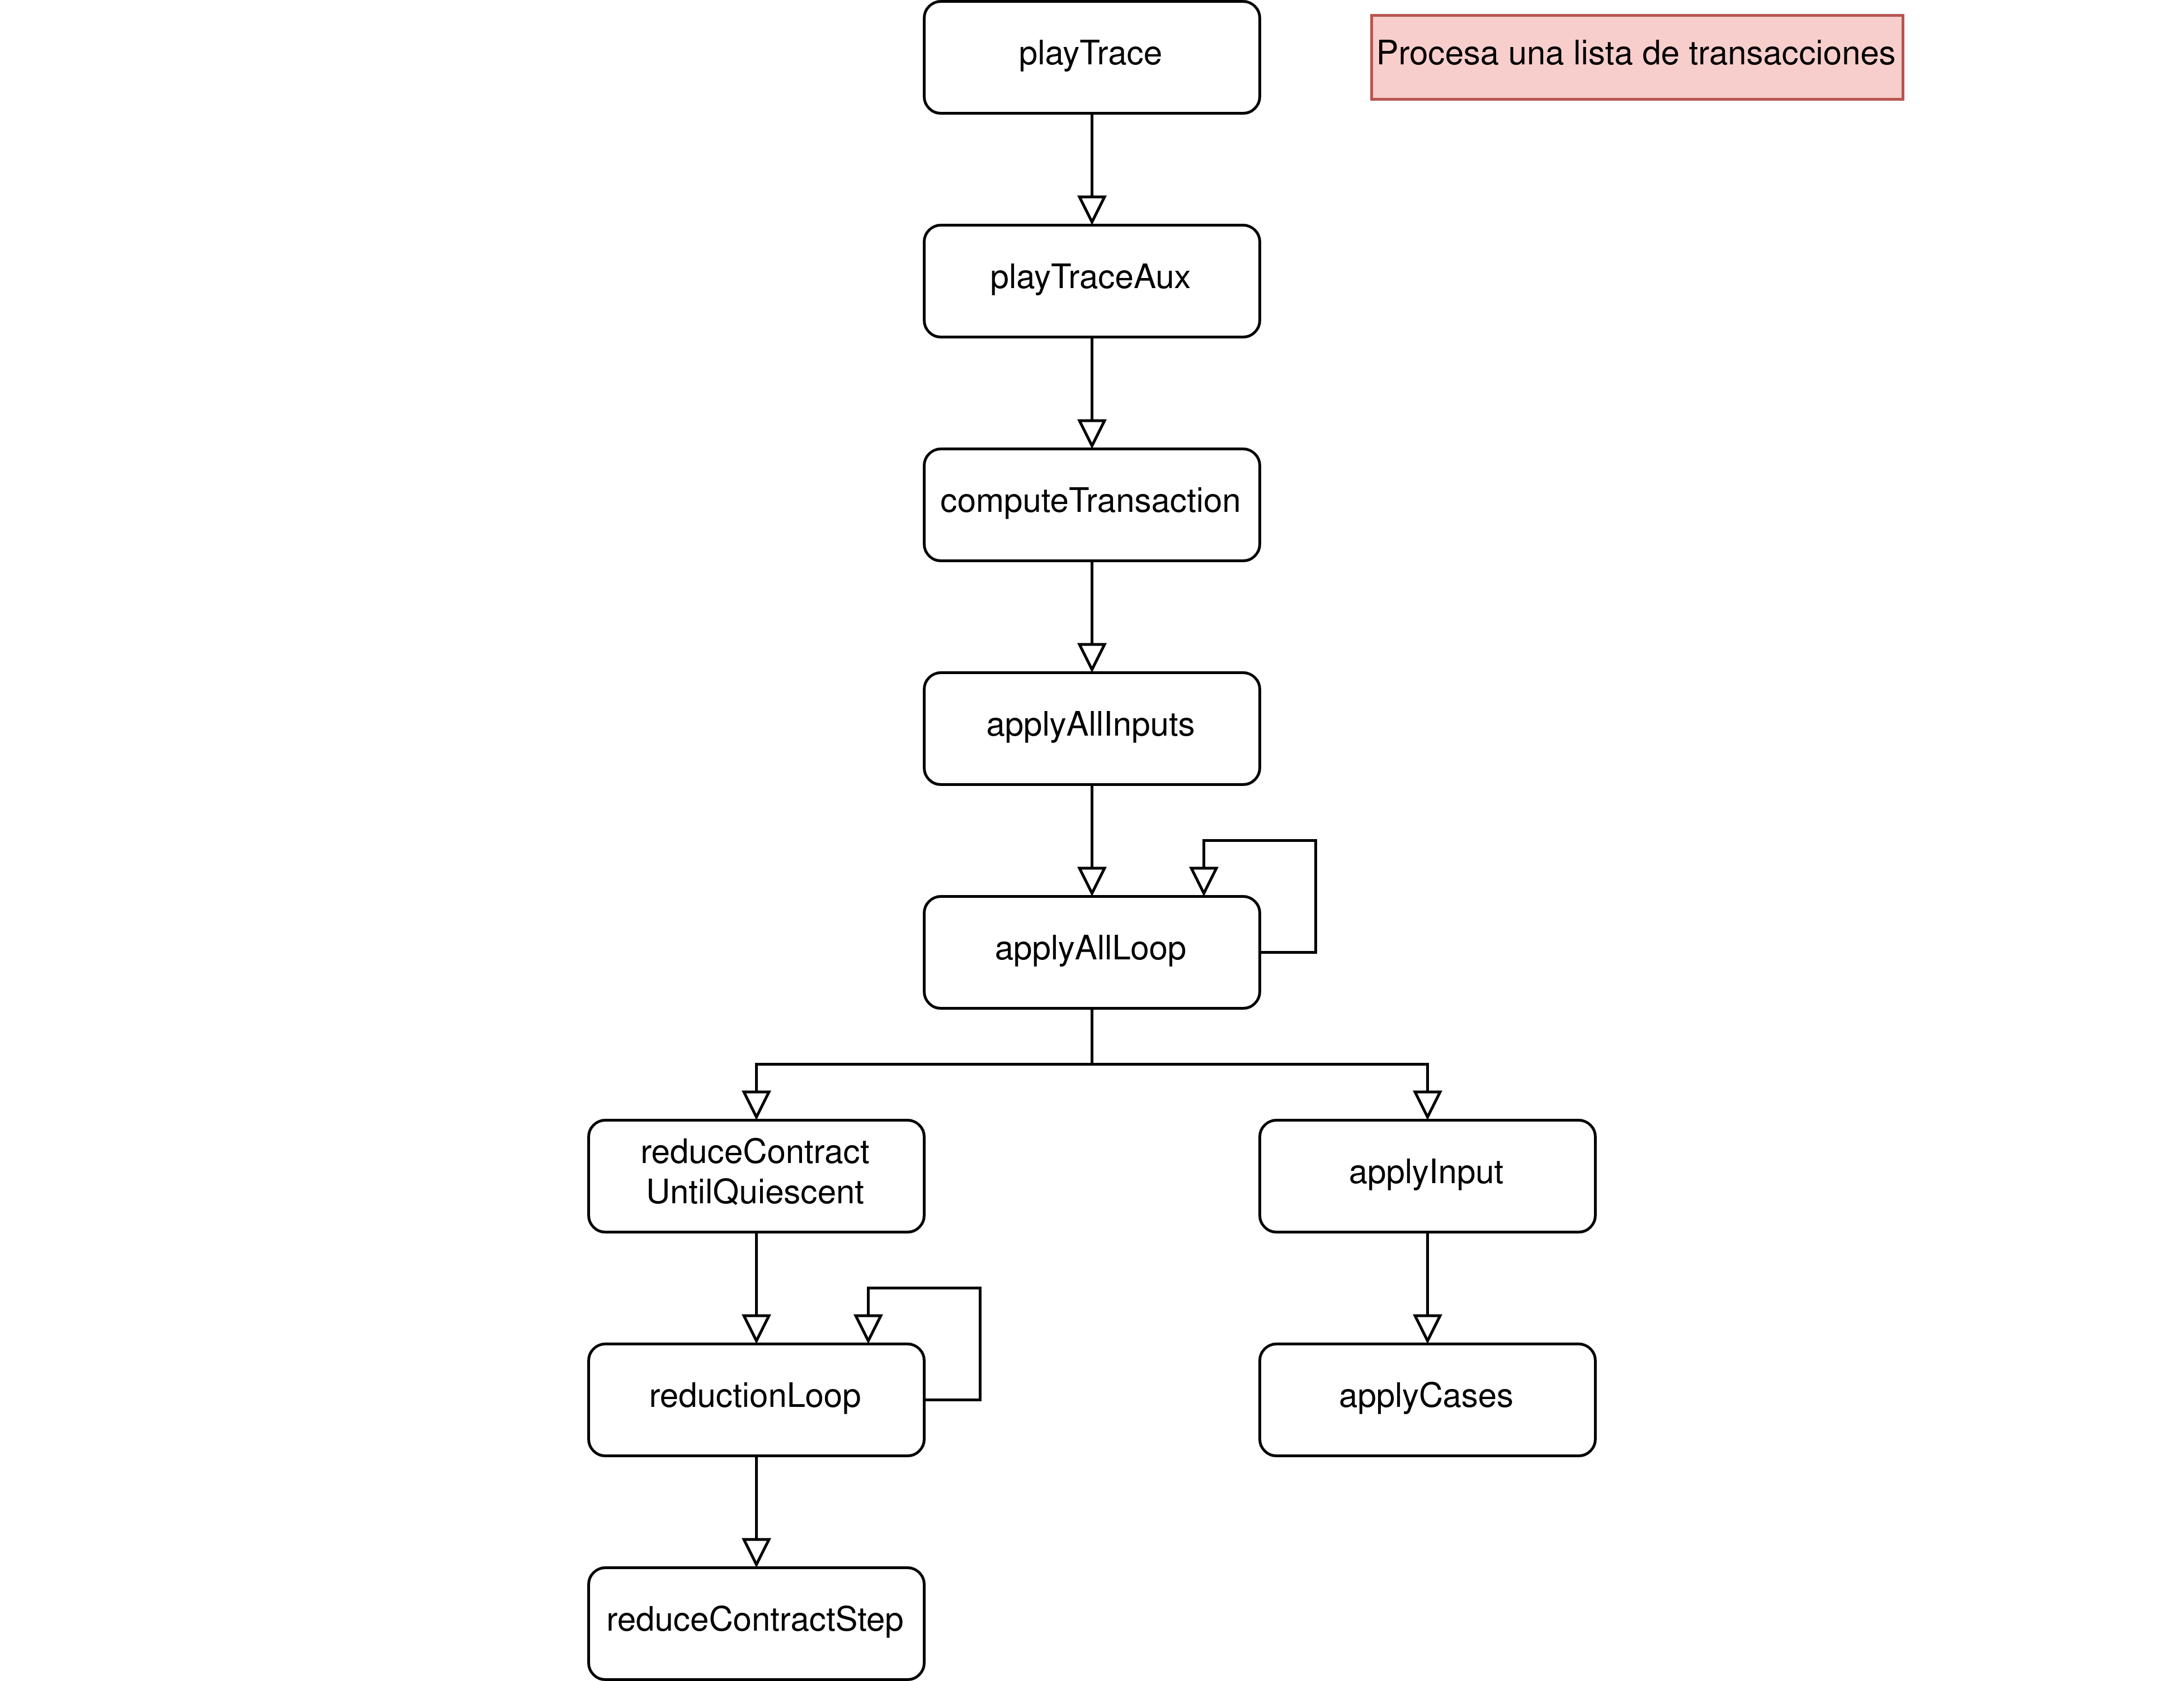
\includegraphics[height=0.8\textheight]{Dependencias_Isabelle_Marlowe_1.png}
    \end{figure}
}
\only<3>{
    \begin{figure}[H]
        \centering
        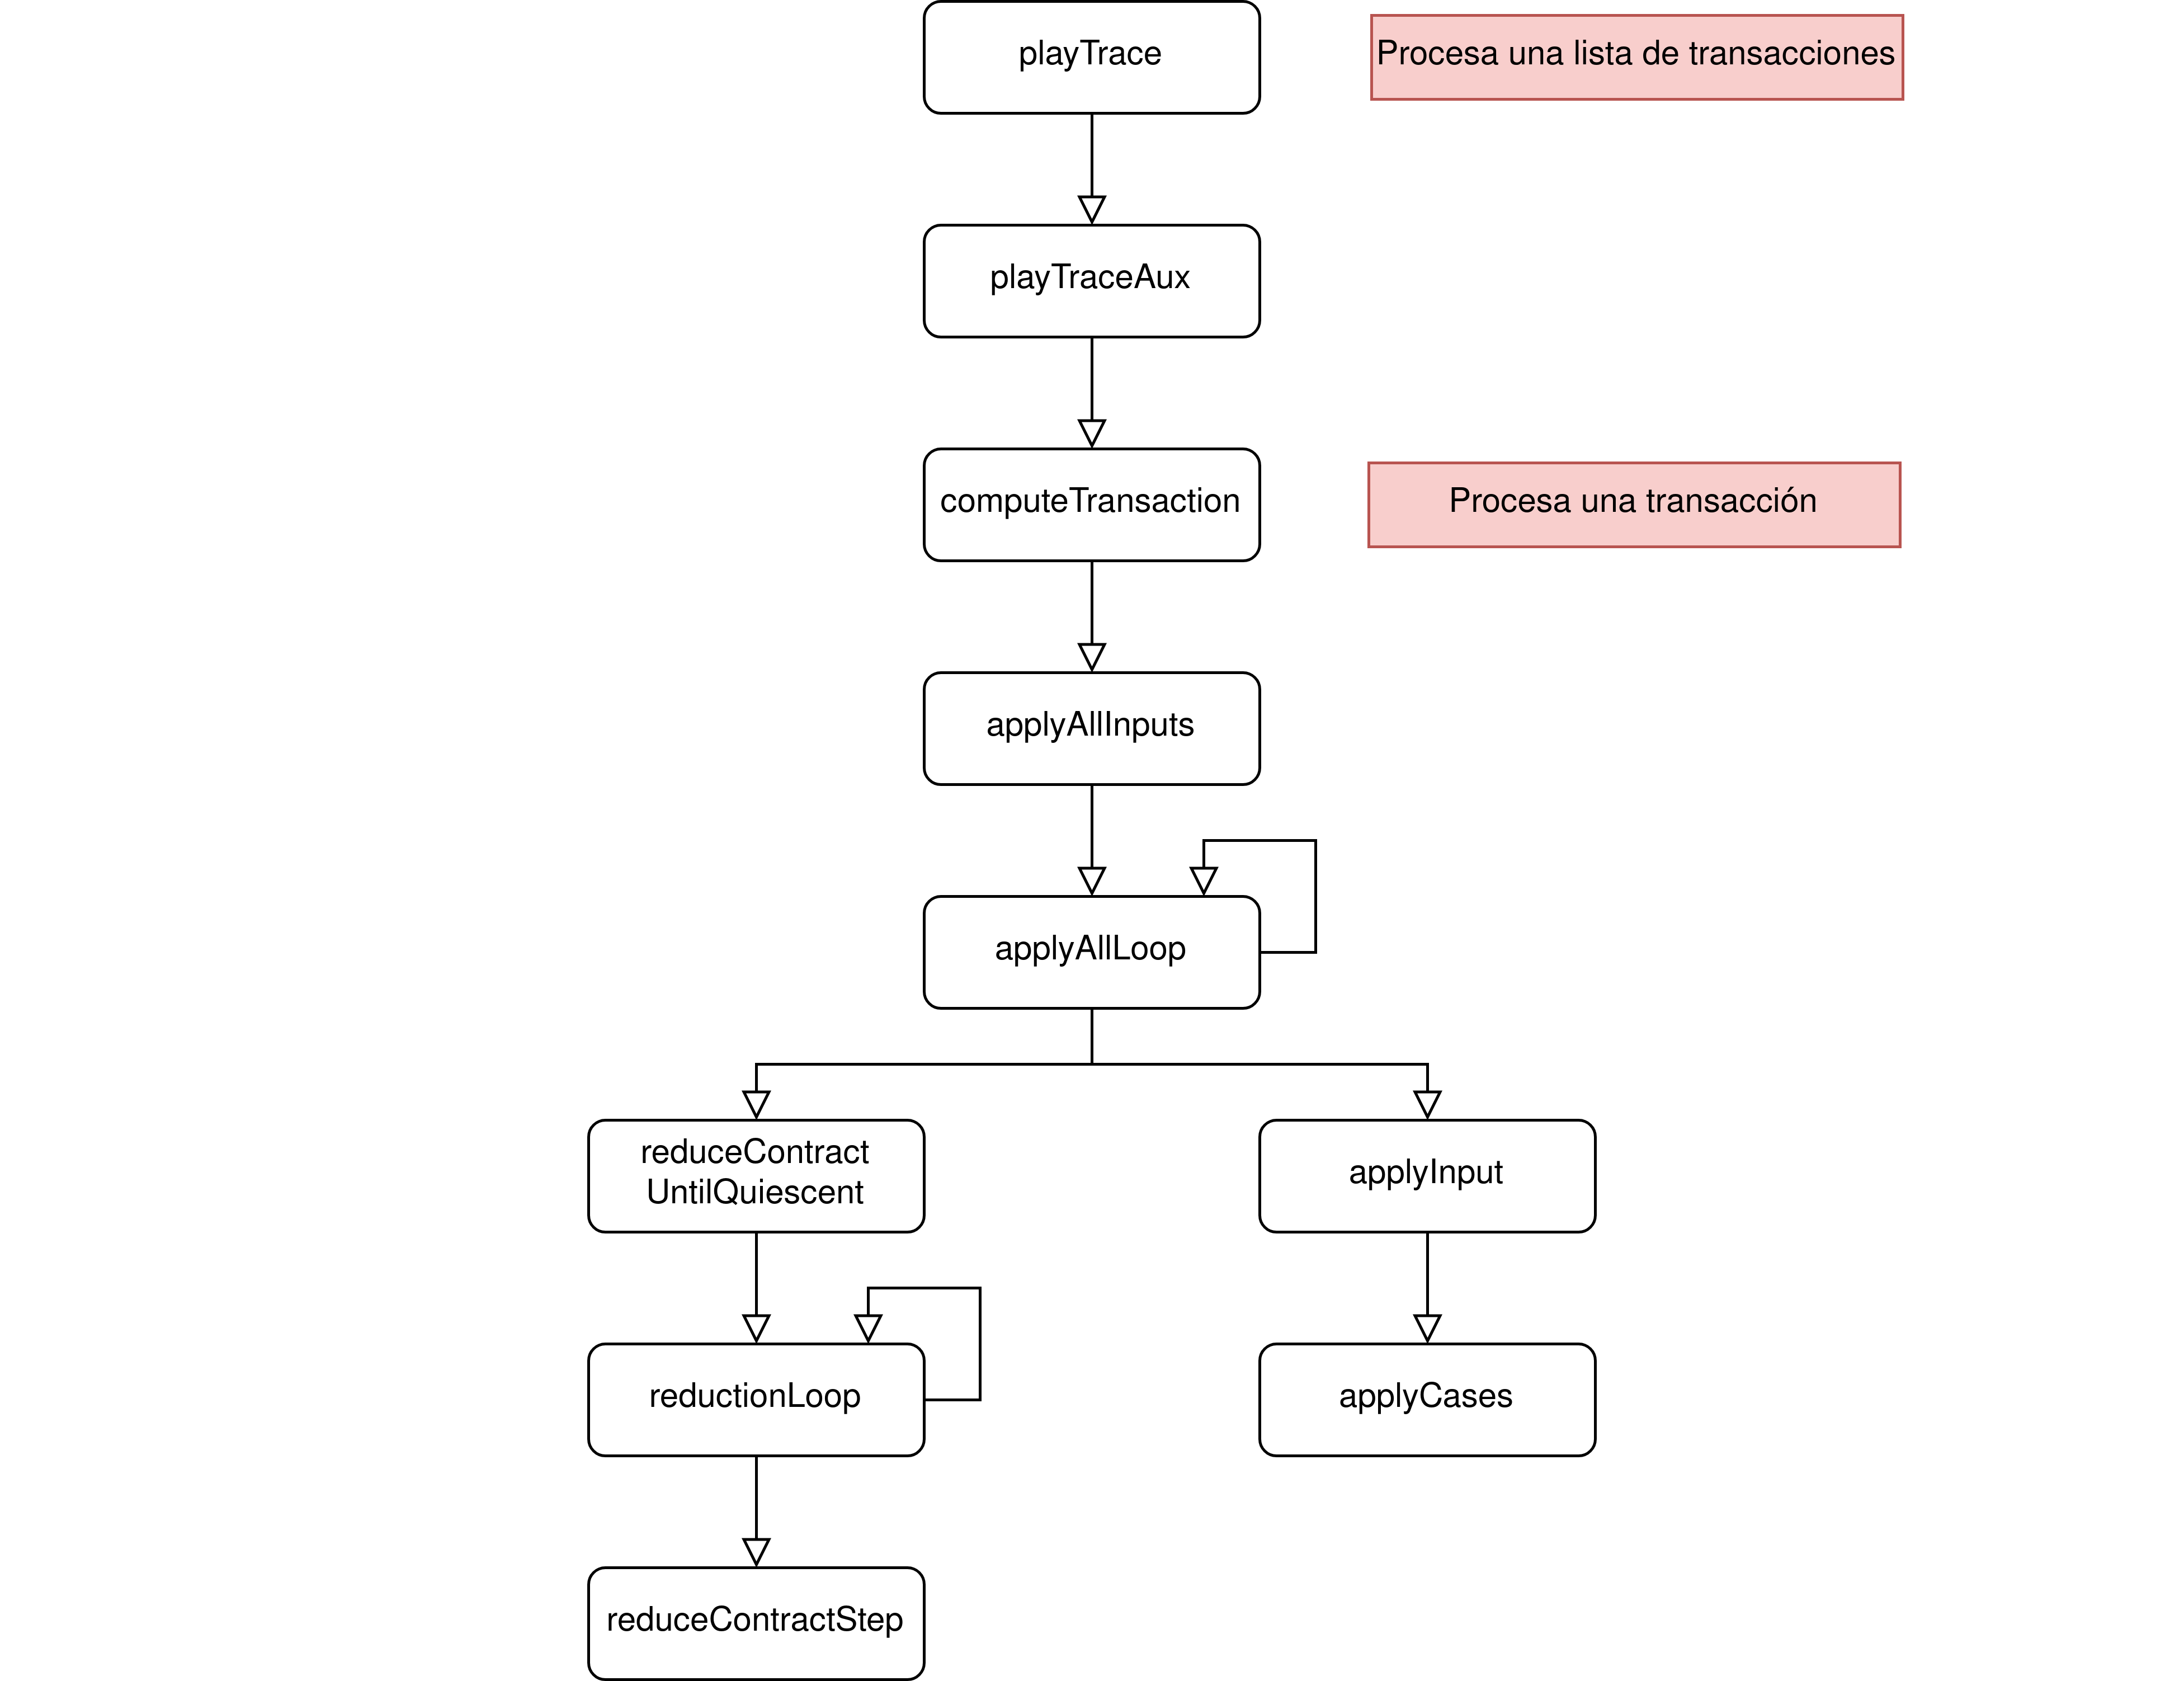
\includegraphics[height=0.8\textheight]{Dependencias_Isabelle_Marlowe_2.png}
    \end{figure}
}
\only<4>{
    \begin{figure}[H]
        \centering
        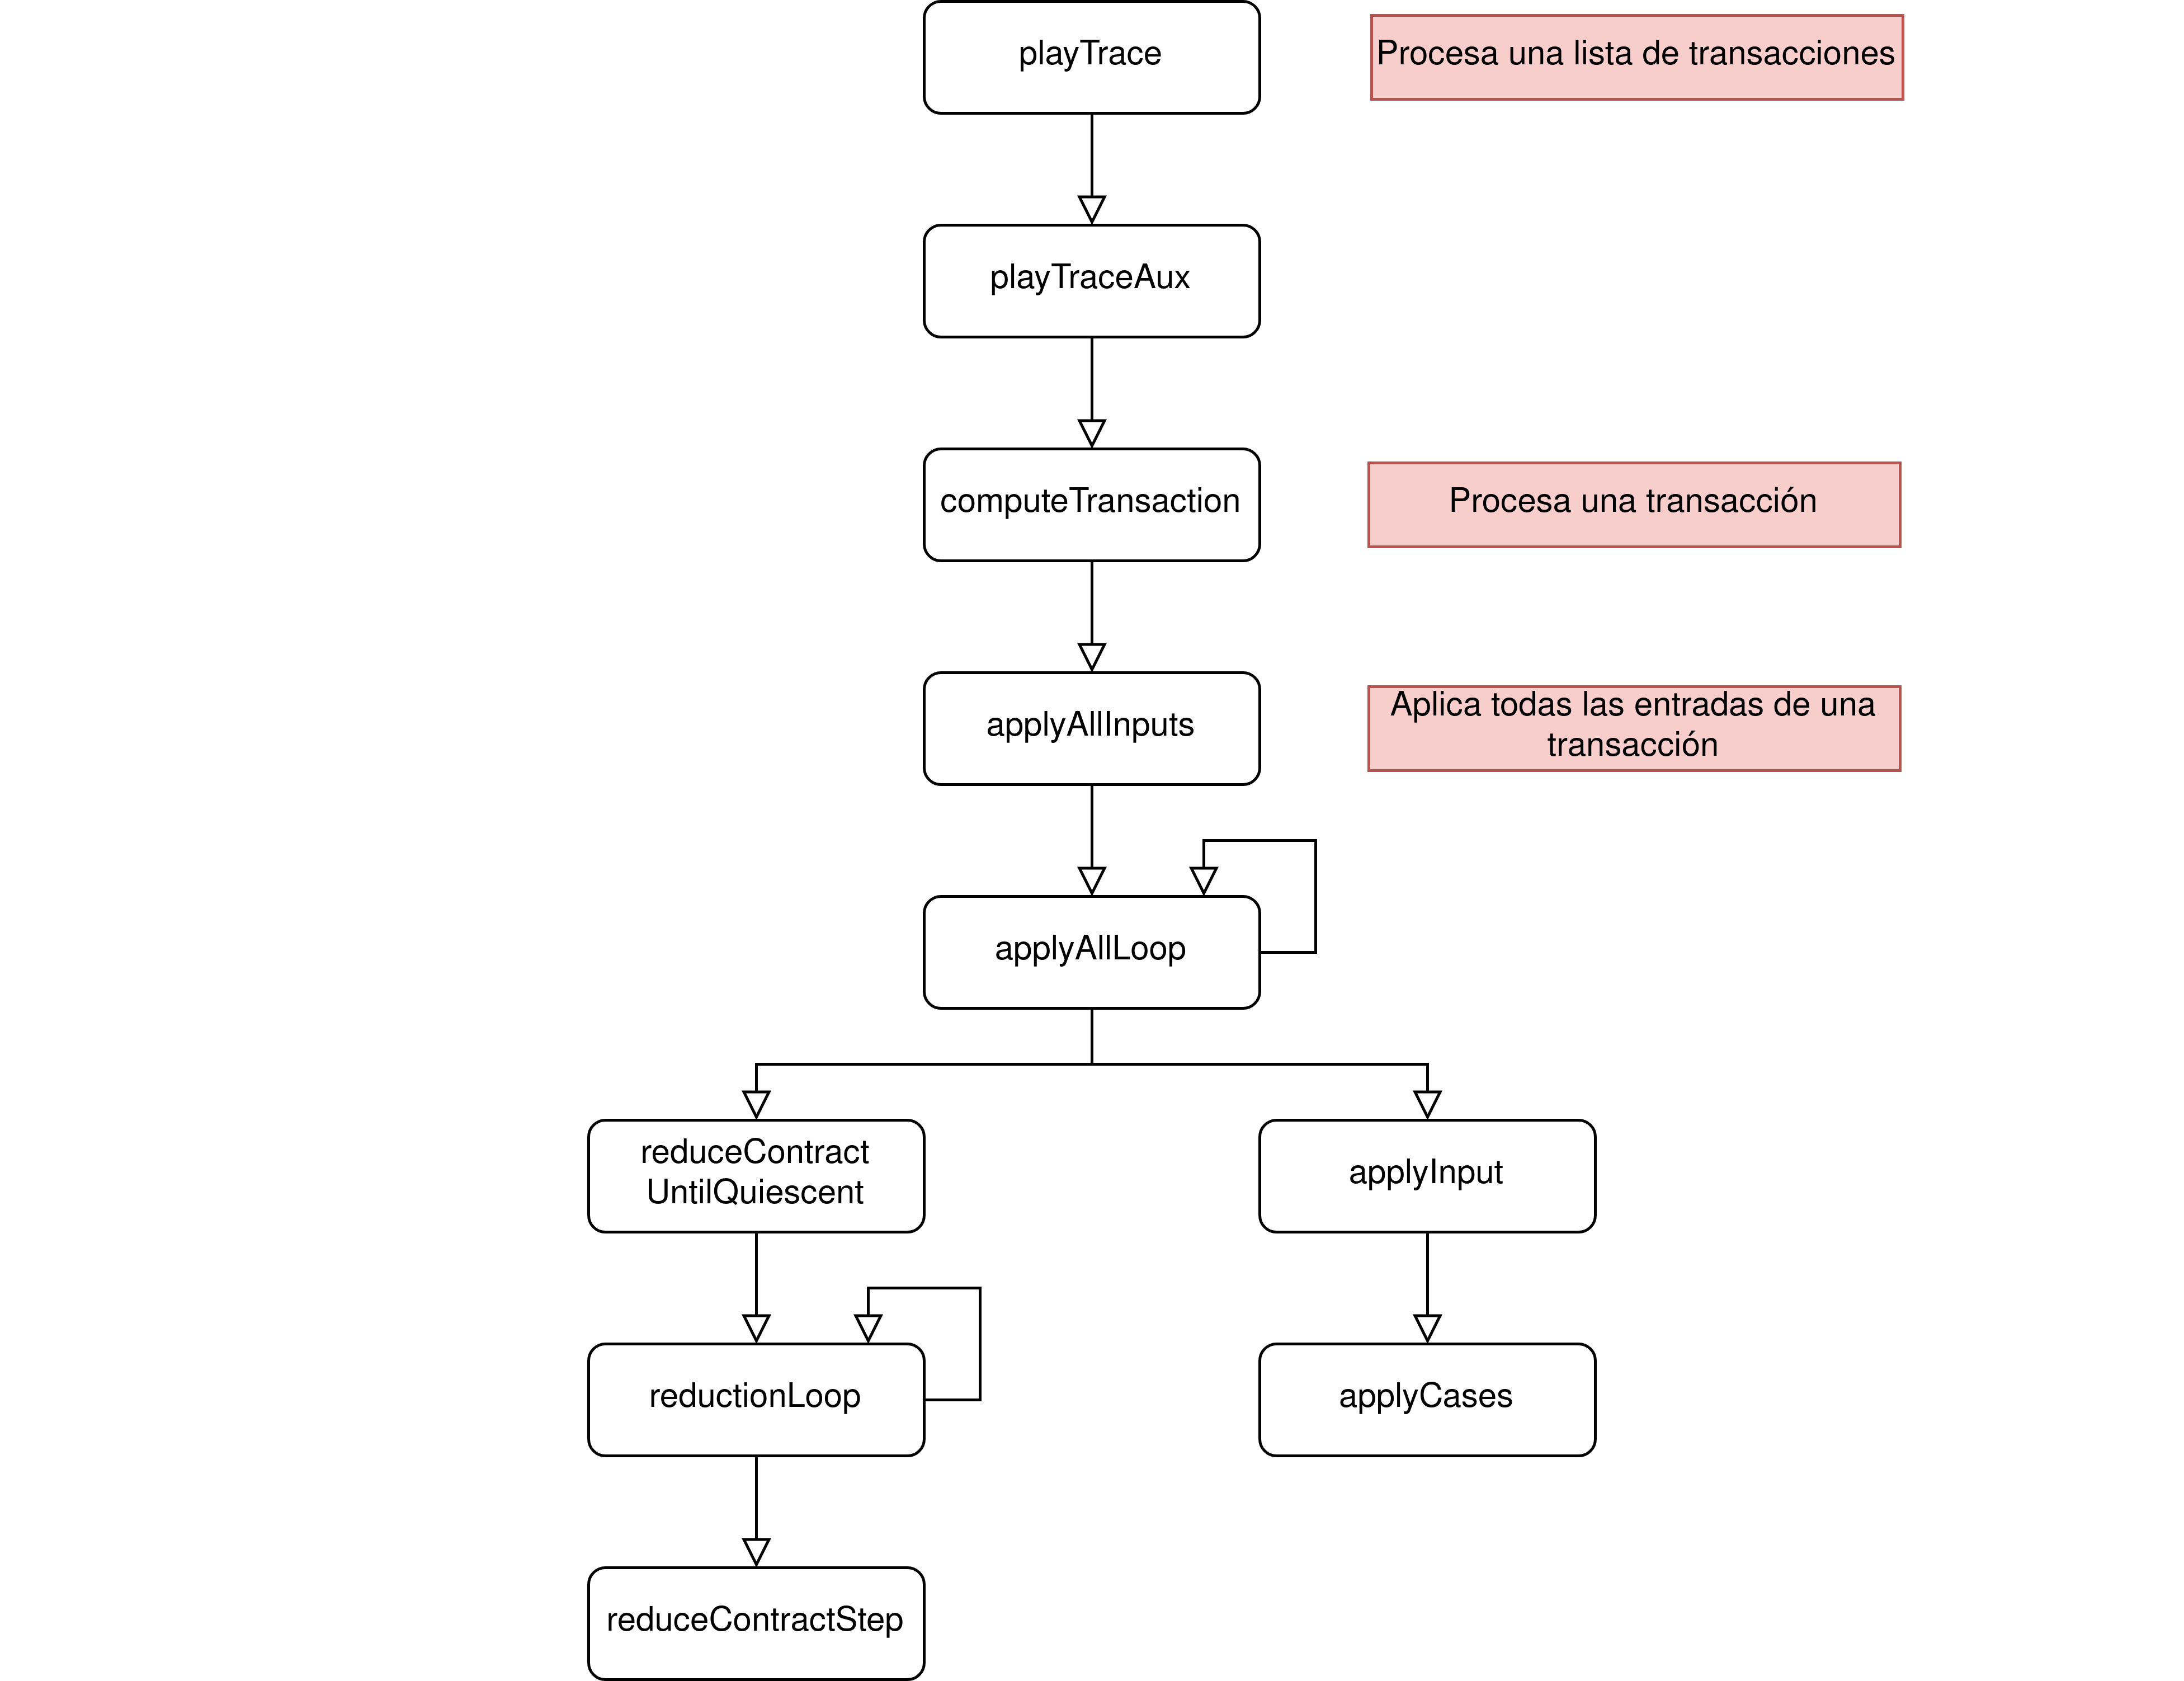
\includegraphics[height=0.8\textheight]{Dependencias_Isabelle_Marlowe_3.png}
    \end{figure}
}
\only<5>{
    \begin{figure}[H]
        \centering
        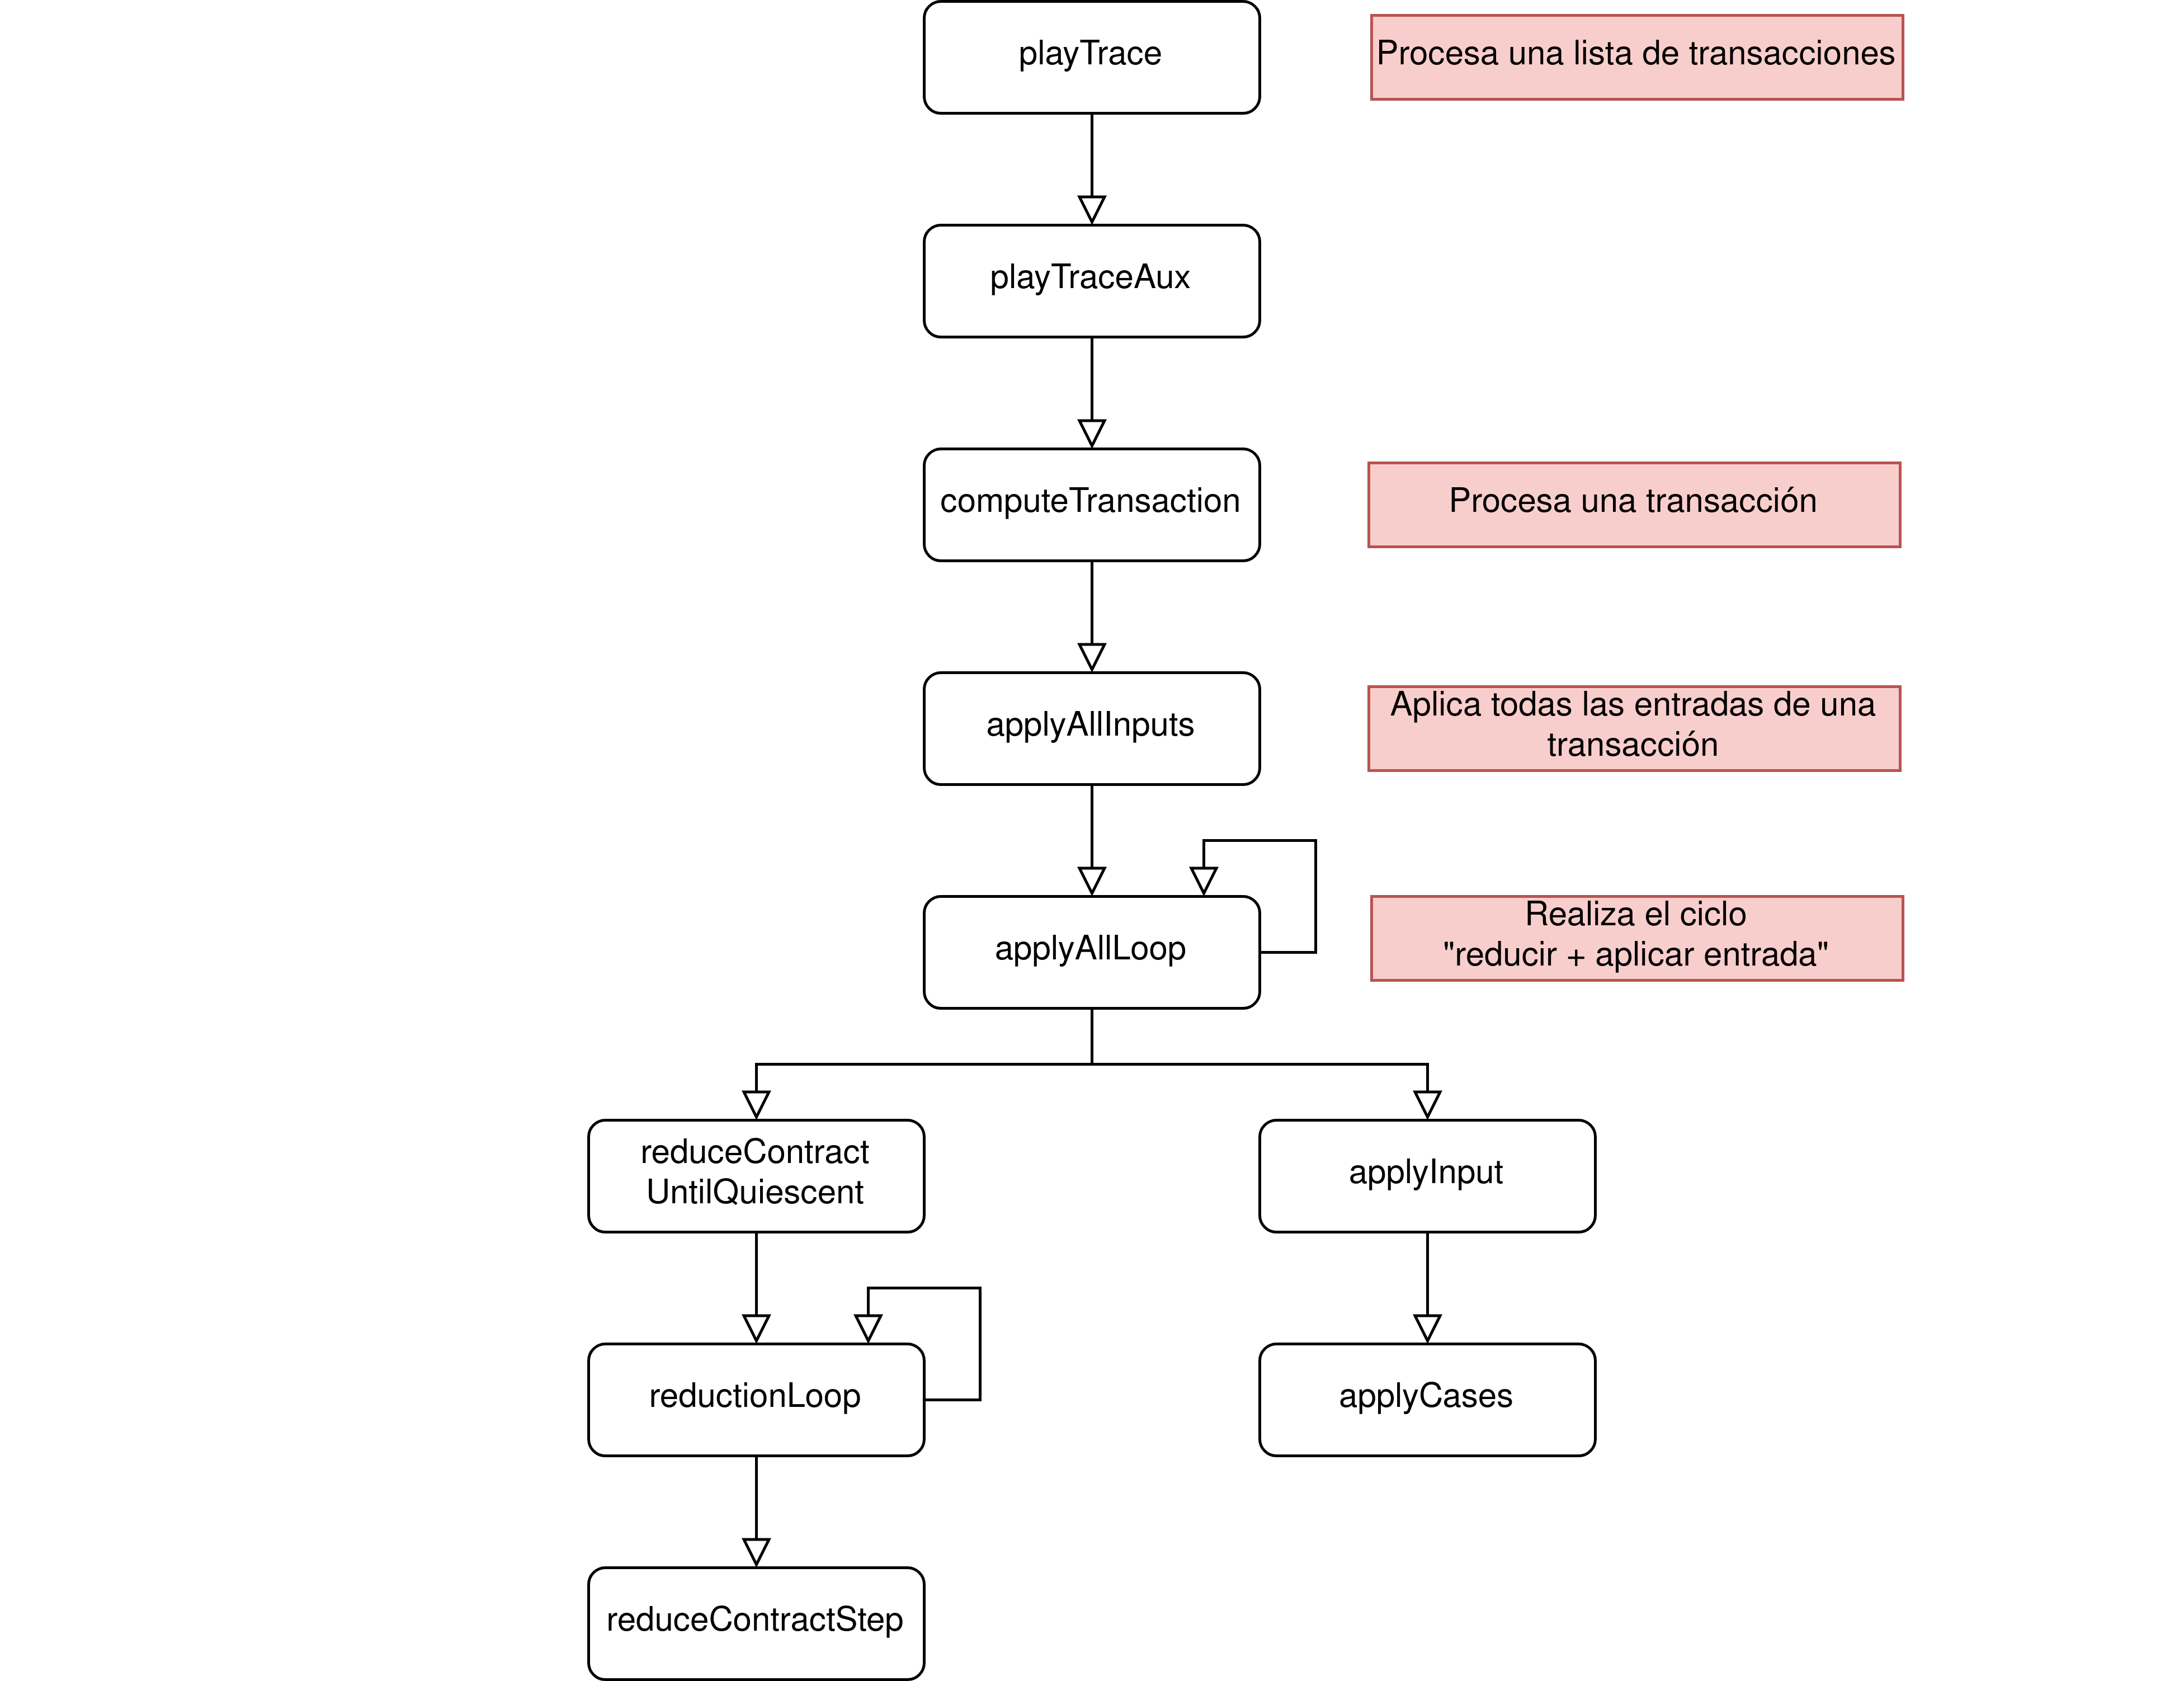
\includegraphics[height=0.8\textheight]{Dependencias_Isabelle_Marlowe_4.png}
    \end{figure}
}
\only<6>{
    \begin{figure}[H]
        \centering
        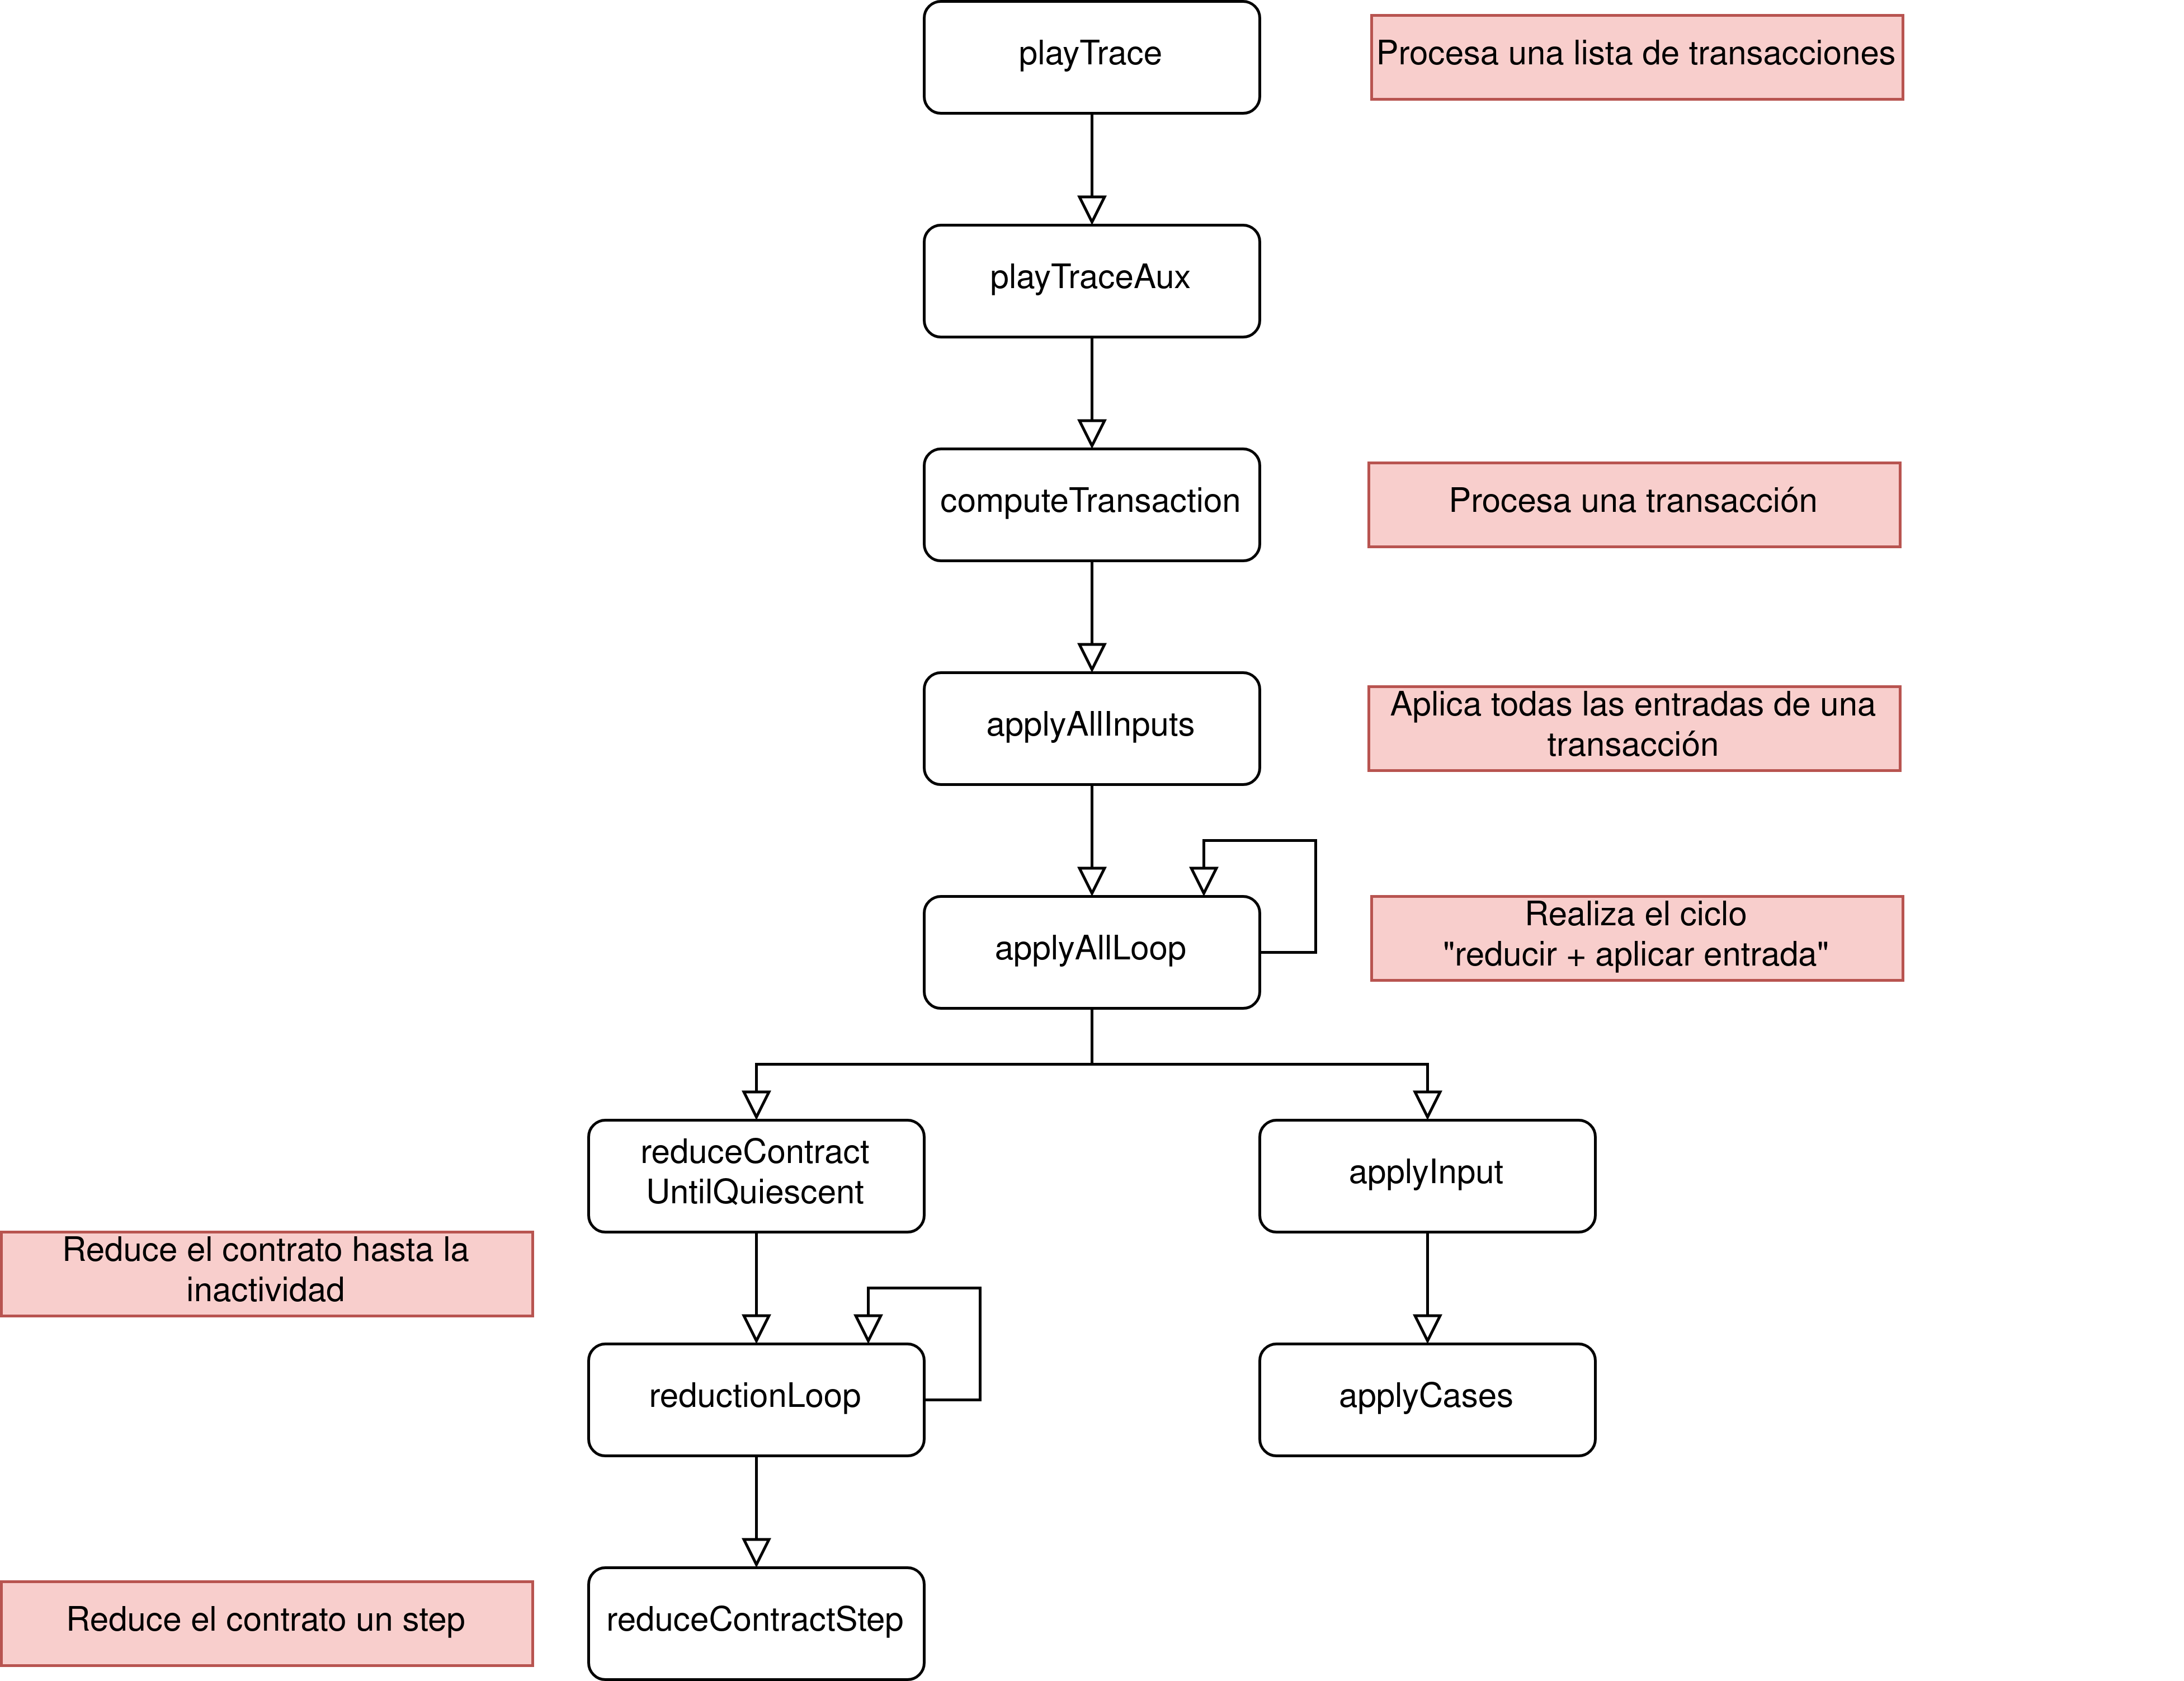
\includegraphics[height=0.8\textheight]{Dependencias_Isabelle_Marlowe_5.png}
    \end{figure}
}
\only<7>{
    \begin{figure}[H]
        \centering
        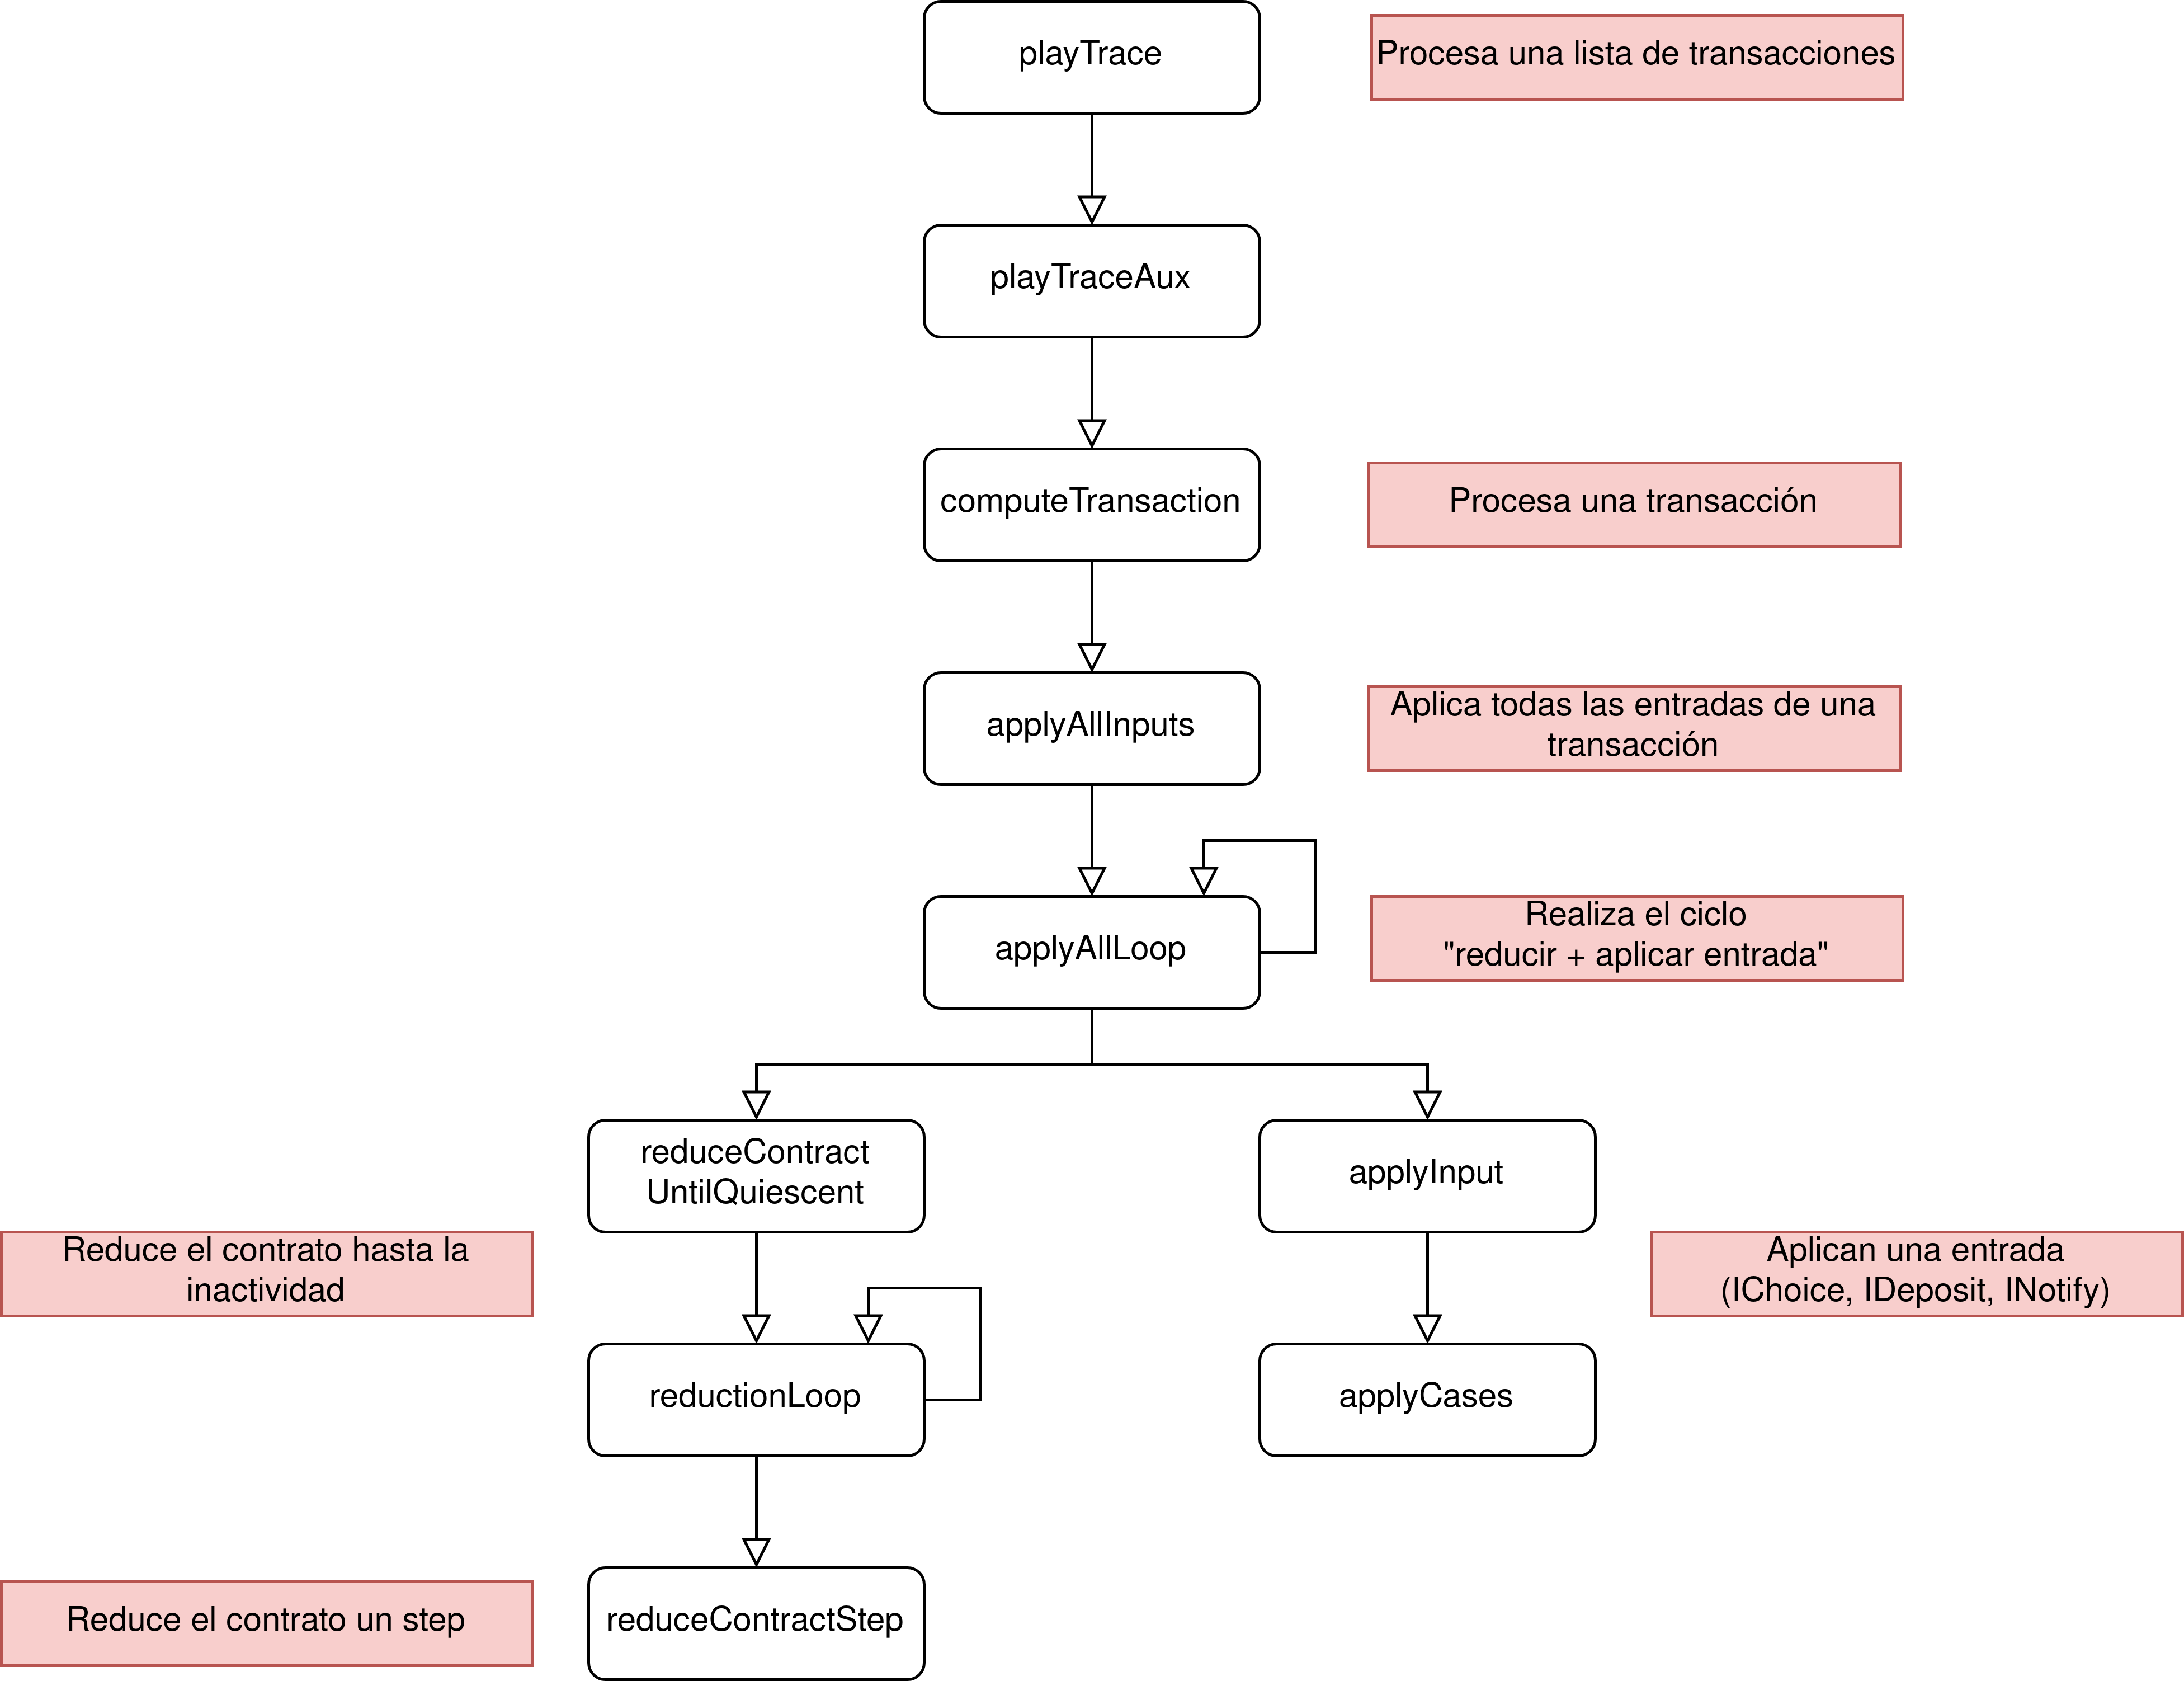
\includegraphics[height=0.8\textheight]{Dependencias_Isabelle_Marlowe_6.png}
    \end{figure}
}


\end{frame}
}




\subsection{Pruebas sencillas sobre contratos específicos}

\begin{frame}{Prueba de \textit{slot} no decreciente en COM}
Supongamos que queremos probar la siguiente propiedad:
\vfill
\begin{quote} 
``\textbf{Evaluar \textit{applyAllInputs} en el contrato COM4}, para cualquier \textit{environment} y \textit{state} dado, \textbf{produce un nuevo estado con \textit{slot} mayor al actual}.''
\end{quote}

\vfill

Este tipo de prueba evita la `vuelta al pasado' por parte del contrato, que podrían llevar a caminos de ejecución no deseados.

\end{frame}

\begin{frame}[fragile]{Prueba del lema de \textit{slot} para un contrato COM.}

Un ejemplo de una propiedad que probé es la siguiente:

\begin{code}{Isabelle}
lemma applyAllInputsDoesNotDecreaseMinSlot :
"applyAllInputs env sta COM4 inputList = 
    ApplyAllSuccess reduced warnings payments newstate cont $\Longrightarrow$
  (minSlot sta) $\leq$ (minSlot newstate)"
  apply auto
  apply (cases inputList)
  apply auto 
  by (smt (z3) ApplyAllResult.distinct(1)
                  ApplyResult.case(1)
                  ApplyResult.case(2)
                  ApplyResult.exhaust
                  COM4_def
                  applyAllLoop_preserves_minSlot
                  applyCases_preserves_minSlot applyInput.simps(1))
\end{code}

\end{frame}

\subsection{Warnings en Auction}

\begin{frame}{El contrato Auction}
Una subasta (\textit{Auction}) es una venta organizada en la cual el comprador (postor) que pague la mayor cantidad de dinero o de bienes a cambio del producto es el ganador de la misma.

\vfill
\pause

En particular, en una subasta basada en una \textit{blockchain}, cada postor debe declarar el dinero primero para convertirse en el mejor postor. Los mismos recuperan su dinero cuando otro postor los supera.


\end{frame}

{\nologo
\begin{frame}

Se puede ver en el siguiente diagrama de secuencia, el comportamiento esperado por la subasta:

\begin{figure}[H]
    \centering
    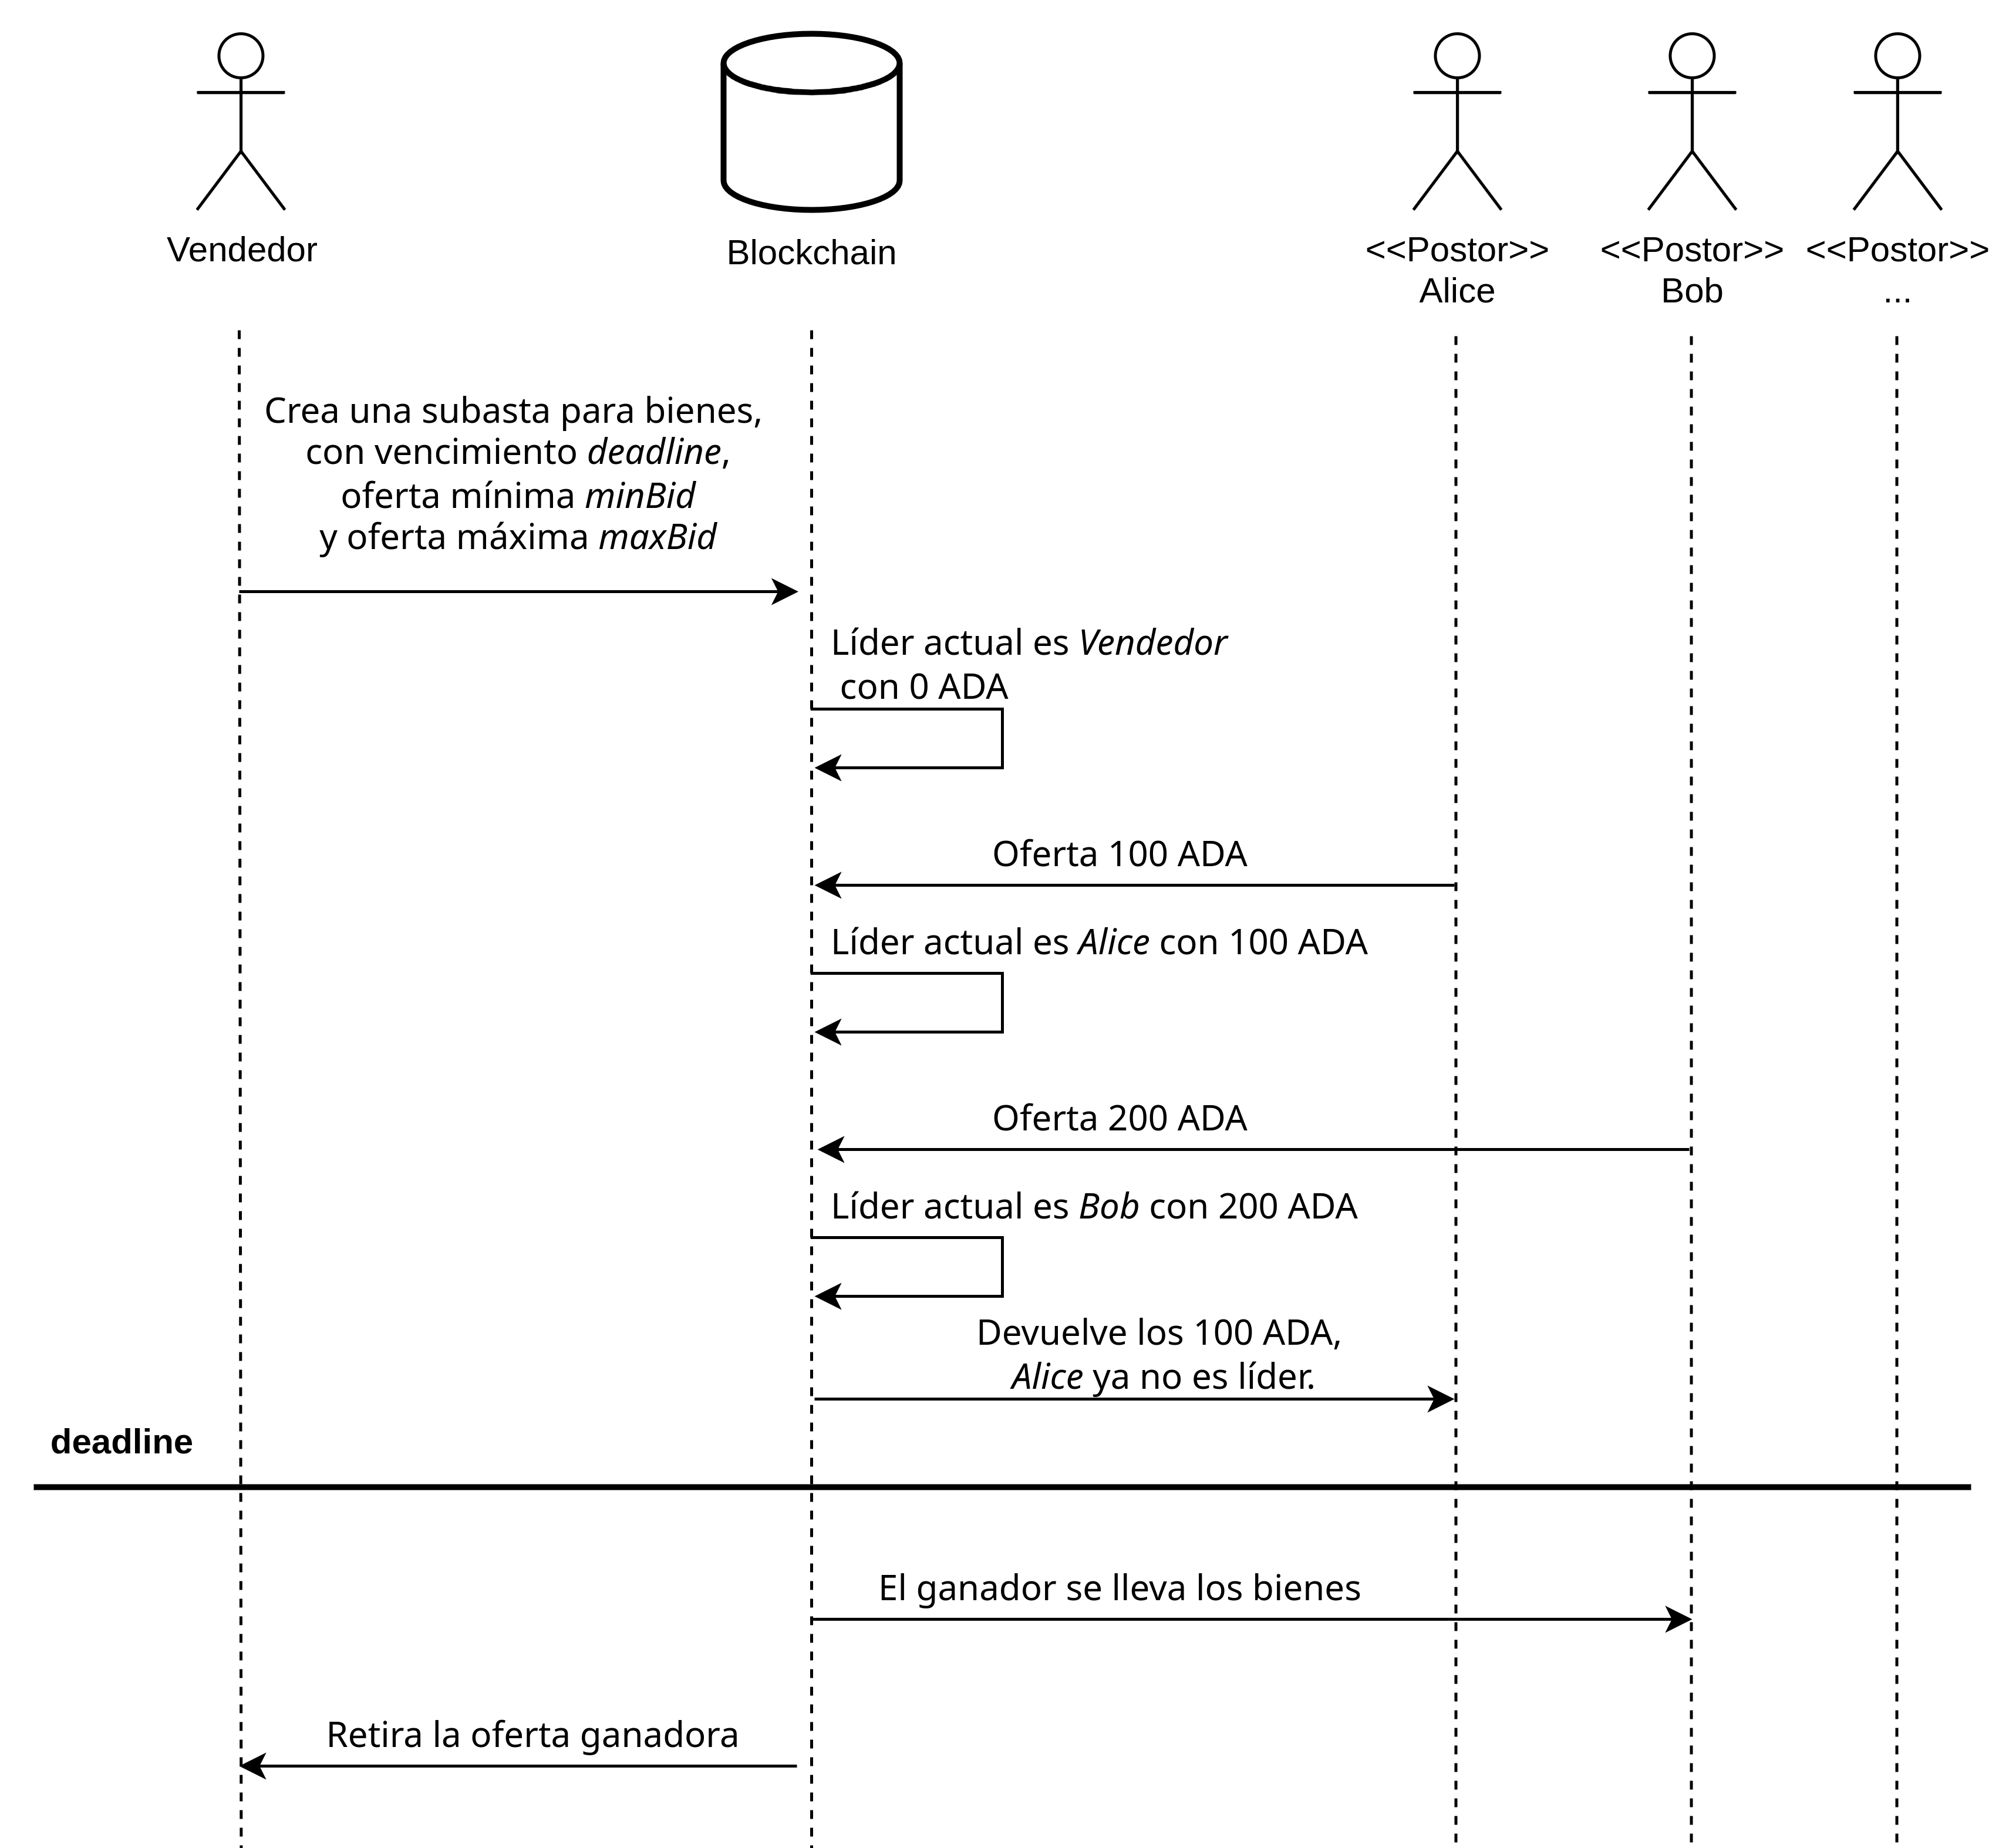
\includegraphics[height=0.8\textheight]{Auction.png}
\end{figure}

\end{frame}
}

\begin{frame}{Pruebas sobre el contrato \textit{Auction}}
Durante parte del desarrollo de mi tesis, probé que \textbf{cualquier contrato Auction no genera advertencias}.

\vfill
\pause

Esto implicó:

\begin{itemize}
    \item \textbf{Traducción} del contrato Auction en Haskell a Isabelle.
        \pause
    \item Prueba de la \textbf{terminación del generador} de contratos Auction.
        \pause
    \item Determinación de una \textbf{invariante} a partir de la cual ningún tipo de \textit{warning} puede ocurrir.
        \pause
    \item Prueba de \textbf{ausencia de Warnings} para todas las funciones involucradas en procesar una transacción.
\end{itemize}


\end{frame}

\begin{frame}{Probando terminación del contrato \textit{Auction}}
Dado que Isabelle/HOL sigue una lógica de funciones totales, la terminación es un requerimiento fundamental. 

\vfill

\textbf{Isabelle intenta probar la terminación automáticamente} cuando se realiza la definición. Pero en algunas circunstancias \textbf{es posible que falle}, y la misma tiene que ser probada manualmente.

\vfill
\pause

La terminación no solo es una propiedad deseable en los contratos, sino que también le \textbf{permite a Isabelle y al usuario utilizar teoremas adicionales}, como por ejemplo el de inducción.

\end{frame}

\begin{frame}[fragile]{Métrica para la terminación}
\begin{code}{Isabelle}
fun evalBoundAuction :: "(contractLoopType + (handleChooseType + handleDepositType)) $\Rightarrow$ nat" where

"evalBoundAuction (Inl (_, ps, qs, _)) =
        2 * length ps + 4 * length qs + 1" |
"evalBoundAuction (Inr (Inl (_, ps, qs, _, p))) =
        2 * length ps + 4 * length qs + (if p $\in$ set qs then 0 else 8)" |
"evalBoundAuction (Inr (Inr (_, ps, qs, _, p))) =
        2 * length ps + 4 * length qs + (if p $\in$ set ps then 0 else 8)"
\end{code}

\end{frame}


\begin{frame}{Invariante para la ausencia de warnings}

Las acciones de los usuarios son imprevisibles y pueden generar \textit{warnings} independientes a la semántica. Algunos ejemplos para este contrato podrían ser:
\vfill

   \begin{itemize}
           \pause
       \item Realizar más de una vez una elección (\textcolor{red}{\textit{ReduceShadowing}}).
           \pause
       \item Ofertar una cantidad negativa (\textcolor{red}{\textit{NonPositiveDeposit}}).
           \pause
       \item Dinero insuficiente en la cuenta para la oferta realizada (\textcolor{red}{\textit{PartialPay}}).
           \pause
       \item Cantidad en el \textit{Pay} no sea positiva o las cuentas tengan suficiente dinero (\textcolor{red}{\textit{NonPositivePay}} y \textcolor{red}{\textit{PartialPay}}).
           \pause
       \item Que el \textit{minBid} del contrato sea positivo, sino se producirá alguna combinación de los \textit{warnings} anteriores.
   \end{itemize} 

\end{frame}

%\begin{frame}
%Esta invariante garantiza la presencia de las siguientes propiedades, que generarían la ausencia de \textit{warnings} al aplicar un \textit{input}:

%\bigskip

%\begin{itemize}
    %\pause
    %\item Que el identificador del \texttt{Let} no exista en el momento en el que se crea (si no se producirá un warning de tipo \textit{ReduceShadowing})
    %\pause
    %\item Que la cantidad en el depósito sea positiva (si no producirá un warning de tipo \textit{NonPositiveDeposit})
    %\pause
    %\item Que la cantidad en el \textit{Pay} sea positiva y además las cuentas tengan suficiente dinero (si no se producirán warnings de \textit{NonPositivePay} y \textit{PartialPay} respectivamente).
    %\pause
    %\item Que \textit{minBid} sea positivo, sino se producirán \textit{warnings} durante las reducciones.
%\end{itemize}


%\end{frame}

{\nologo
\begin{frame}[fragile]{Definición en Isabelle de la invariante para \textit{Auction}}
Es por eso que se formularon una serie de \textbf{pre-condiciones o invariantes que deben ser satisfechas} para poder asegurar que el contrato no genera \textit{warnings}.

\vfill

\begin{code}{Isabelle}
definition invariantHoldsForAuction :: "AuctionTerms $\Rightarrow$ AuctionWinner $\Rightarrow$ Party list $\Rightarrow$ Party list $\Rightarrow$ State $\Rightarrow$ bool" where

"invariantHoldsForAuction terms m ps qs curState =
       (($\forall$ x . x $\in$ set qs $\longrightarrow$
                $\neg$ member (partyToValueId x) (boundValues curState))
     $\land$ ($\forall$ x . x $\in$ set ps $\longrightarrow$ 
                findWithDefault 0 (partyToValueId x) (boundValues curState) > 0)
     $\land$ ($\forall$ x y . m = Some (x, y) $\longrightarrow$ 
              ((lookup (y, token_ada) (accounts curState) = 
                lookup (partyToValueId y) (boundValues curState))
             $\land$ (findWithDefault 0 (partyToValueId y) (boundValues curState) > 0) 
             $\land$ (UseValue (partyToValueId y)) = x))
     $\land$ (minBid terms > 0))"
\end{code}

\end{frame}
}

{\nologo
\begin{frame}[fragile]{Ausencia de warnings en Isabelle al computar una transacción}
\begin{code}{Isabelle}
lemma auctionIsSafe_computeTransaction :
    "invariantHoldsForAuction terms m ps qs sta $\Longrightarrow$
     computeTransaction tra sta (contractLoop m ps qs terms) =
       TransactionOutput trec $\Longrightarrow$ txOutWarnings trec = []"

  using fixingIntervalPreservesInvariant auctionIsSafe_computeTransactionFixSta
  by (smt (verit, ccfv_SIG) IntervalResult.simps(6) closeIsSafe computeTransaction.simps fixInterval.elims)
\end{code}

\vfill

Esta prueba depende de las demostraciones previas sobre todas las funciones en las que depende (\textit{ApplyAllInputs}, \textit{ReductionLoop}, \textit{ReduceContractStep}, \textit{ApplyInput}, etc.)

\end{frame}
}

\section{Posibles temas de desarrollo futuro}

{\nologo
\begin{frame}{Posibles temas de desarrollo e investigación}
    \begin{itemize}
        \item Con respecto a la escritura de contratos ACTUS en Cardano, actualmente \textbf{no se han terminado de escribir todos los contratos especificados por el estándar}.

            \pause
            \vfill

        \item En cuanto a la verificación de programas, es posible \textbf{tomar algunos contratos} (por ejemplo entre los ejemplos del \textit{Playground}) \textbf{en los que no se esperan warnings y verificarlos} mediante Isabelle. 

            \medskip
            
            Dichas verificaciones podrán beneficiarse de los lemas y técnicas utilizadas para los contratos \textit{Auction} y \textit{Close}.

            \pause
            \vfill

        \item La \textbf{traducción automática de algunas sentencias de código Haskell a Isabelle}. Parte de esta idea es abarcada en~\cite{translating-haskell-to-isabelle}, aunque manteniendo la traducción manual.
    \end{itemize}
\end{frame}
}

\begin{frame}
\begin{center}
    \Huge ¿Preguntas?
\end{center}
\end{frame}

\begin{frame}<0>[noframenumbering]
    \bibliographystyle{apalike}
    \bibliography{bibliografia.bib}
\end{frame}

\end{document}
